\documentclass[a4paper,oneside]{memoir}
\usepackage[T1]{fontenc}
\usepackage{textcomp}
\usepackage[utf8]{inputenc}
\usepackage[danish]{babel}
\usepackage[garamond]{mathdesign}
\usepackage{url}
\usepackage{graphicx}
\usepackage{pdflscape}
\usepackage{longtable}
\usepackage[draft]{fixme}
\usepackage{hyperref}
\usepackage{memhfixc}
\usepackage{listings}
\usepackage{amsmath}

\DeclareTextFontCommand{\textfleur}
{\fontencoding{T1}\fontfamily{FleurCornerCaps}\selectfont}


\renewcommand{\ttdefault}{pcr} % bedre typewriter font
\renewcommand{\rmdefault}{ugm} % garamond

\textheight = 625pt
\textwidth = 400pt
\oddsidemargin = 25pt


\lstloadlanguages{HTML}
\lstset{language     = ML,
        extendedchars= true,
        breaklines   = false,
        tabsize      = 2,
        showstringspaces = false,
        basicstyle   = \small\ttfamily,
        commentstyle = \em,
        inputencoding= utf8
      }


\usepackage{lettrine}

%\overfullrule=5pt

%\setsecnumdepth{part}

\title{Hjemmesideanalyse  \\ \small{Førsteårsprojekt}}

\author
{
  Gruppe 1:\\
  Troels Henriksen (athas@sigkill.dk)\\
  Jesper Reenberg (reenberg@kampsax.dtu.dk)\\
  Martin Dybdal (dybber@dybber.dk)\\ \\
  Vejledere: Dina og Kasper
}


\setcounter{tocdepth}{2}
\setcounter{secnumdepth}{2}

\pagestyle{plain}
\chapterstyle{hangnum}
\date{\today}

\begin{document}
\maketitle
\newpage
\tableofcontents*

\chapter{Indledning}
\label{indledning}
Mange hjemmesider forfattes i dag uden omtanke for om sidens målgruppe
er i stand til at læse sidens indhold --- det sproglige niveau er
ganske enkelt for højt (eller for dårligt, om man vil). Ydermere
forfattes indholdet af mange hjemmesider med primitive værktøjer
(f.eks. simple tekstfelter direkte på siden, eller simple
skriveprogrammer), der mangler de hjælpefunktioner som findes i
almindelige skriveprogrammer. Dette resulterer i at hjemmesider ofte
indeholder flere stavefejl end konventionelle tekster. Disse mangler
kan gøre hjemmesider sværere at bruge for den tilsigtede målgruppe, og
derved reducere deres effektivitet, ligegyldigt hvad målet med siden
så end er.

Baseret på denne problemstilling har vi implementeret et program,
designet til at bistå hjemmesideforfattere med at forbedre den
sproglige kvalitet af deres sider, hvad enten dette er ved at reducere
antallet at stavefejl eller at omskrive unødigt kompliceret tekst.

Denne rapport beskriver design- og implementeringsprocessen bag vores
løsning af problemet, en arbejdsproces der blev udført i forbindelse
med Førsteårsprojektet på DIKU i blok 4, 2007.

Vores program endte med at opfylde alle de vigtigste krav nævnt i
vores kravspecifikation, og tests og eksperimenter viste at det er i
stand til at udføre de opgaver vi kom frem til i vores analyse (se
sektion \ref{analyse}). For nærmere detaljer omkring programmets
endelige tilstand, se konklusionen i sektion \ref{konklusion}.

Det forventes at læseren af denne rapport har en hvis grad af teknisk
kompetence, har erfaring med programmering og har en overordnet
forståelse for sproget HTML\footnote{Et sprog der bruges til at
  beskrive struktur og indhold af websteder}.

\section{Terminologi}

Herpå følger definitionen af enkelte begreber brugt i denne rapport.

\begin{description}
\item[Websted ---] en samling HTML-sider placeret på samme domæne. Et
  websted indeholder én eller flere \textit{sider}.
\item[Side ---] en enkelt HTML-side på et websted.
\item[Sidesværhedsgrad ---] et tal der angiver hvor svær en given side er
  at læse.
\end{description}

\chapter{Problemformulering}
\label{problemformulering}
Formålet med projektet er at skabe et program der kan bistå med at
forøge læsbarheden og den tekstmæssige kvalitet af hjemmesider. Af
simplicitetshensyn understøtter vi kun sider primært skrevet på dansk,
og vi behandler kun hjemmesidens indhold, og ikke dens typografi og
design.

Baseret på en analyse af hvilken målgruppe et sådan program er bedst
egnet til vil vi udvælge en mængde af features, som vi både mener er
realistiske at implementere på den afsatte tid, og som vil være
brugbare for projektets målgruppe. Bl.a. har vi tænkt os at inddrage
den semantiske information HTML giver omkring en sides tekst til at
give en mere præcis vurdering af dens læsbarhed.

\chapter{Analyse}
\label{analyse}
I dette afsnit vil vi beskrive de tanker vi gjorde os omkring
problemet, og de forskellige løsningsmuligheder vi vurderede.

\section{Målgruppe}
\label{målgruppe}
Der er adskillige mulige målgrupper en løsning på problemet kunne være
orienteret imod --- fra hjemmebrugere der skriver personlige sider,
over individuelle skribenter på et større websted til selve
webmasteren på en stor side. Ydermere kan et websteder indhold
fortolkes på flere forskellige måder --- enten som almindelig tekst
omgivet af HTML--data uden betydning, eller med et forsøg på at
benytte den information som HTML--strukturen udtrykker. Sidstnævnte
gør det væsentligt lettere for et program at undersøge indholdet på et
websted, idet mere information om sidernes indhold så er eksplicit
udtrykket i sidernes kode, i stedet for at programmet skal
``gætte''. Dette har også relevans i forhold til målgruppen, idet
HTML's avancerede features for at udtrykke semantisk information
omkring teksten (information om sprog, forkortelser, osv) primært
benyttes af tekniske brugere, og det virker paradoksalt at lave en
løsning til ikke-tekniske brugere der fungerer bedst med data
produceret af tekniske brugere. Idéen er jo ikke blot at brugeren skal
kunne køre en analyse, men også derefter foretage rettelser på
baggrund af analyseresultatet, og derfor går vi ud fra at brugeren
kører programmet på websteder som vedkommende selv har mulighed for at
ændre. Vi besluttede os for at det ville være et spild at undlade at
udnytte HTML's muligheder for at angive semantisk information omkring
teksten, men da en så lille del af verdens websteder benytter sig af
HTML's muligheder indenfor dette område, ville det heller ikke være
hensigtsmæssigt at handikappe programmet til kun at virke acceptabelt
på denne form for HTML. Vores endelige målgruppe endte med at blive
todelt --- webmastere og (semi--)professionelle skribenter. Dette valg
baserer vi på at både webmastere og skribenter har en stor interesse i
at deres sider eller tekst er let at læse, og har motivation til at
sætte sig ind i hvorledes man skriver god HTML, og derved gør det
muligt for et program at foretage en så god undersøgelse af webstedet
som muligt.\footnote{Det kan nævnes at HTML-sider rig på semantisk
  information også gør det lettere for brugere af alternative
  weblæsere, som f.eks. blinde der benytter sig at netoplæsere, at
  benytte sig af siden} De, der ikke har interesse eller motivation
til at sætte sig ind i teknikken, har sandsynligvis også mindre
interesse i at deres websteder er lette at læse --- ejerne af
professionelt orienterede websteder har en væsentligt større interesse
i at deres sider er let læsbare end forfatterne af f.eks. en families
hjemmeside.

I vores kravspecifikation er målgruppen defineret endnu løsere, som en
person bekendt med HTML som har en professionel interesse i at
webstedet er læsbart. Dette er hvilke brugere vi ønsker at programmet
skal kunne \textit{benyttes} af, men programmet er optimeret mod at
fungere bedst i de ovenfor nævnte scenarier med de nævnte
brugergrupper.

\section{Overvejelser omkring brugsscenarier}
\label{brugsovervejelser}
Vi blev hurtigt enige om at det er langt mere interessant at analysere
et websted som helhed, end kun at analysere en specifik HTML--side, og
samtidigt at det er en nødvendighed at løsningen kan gennemgå
(``crawle'') et online websted, og ikke være afhængig af at det i
forvejen er hentet og er beliggende som filer på brugerens
harddisk. Årsagen til denne beslutning er bl.a. at hvor det er
relativt nemt at få et program, der kan analysere et helt websted, til
kun at analysere en enkelt side, er det omvendte langt sværere, idet
man så skal implementere crawling separat fra programmet. Ydermere er
især den ene del af vores målgruppe --- webmastere --- sandsynligvis
langt mere interesserede i at analysere hele det websted de er
ansvarlige for, for at finde ud af hvilke undersider der er
uacceptabelt svære at læse, end at analysere enkeltsider. Idet vi let
kan forestille os at det kan tage lang tid at analysere alle
undersider på et stort websted, forestiller vi os også et brugsmønster
hvori programmet automatisk bliver kørt med et fast interval, og
producerer et resultat som er tilgængeligt for alle der arbejder på
siden. Dette er langt mere effektivt end at alle skribenter hver især
skal køre tidskrævende analyser hver for sig. Dog opfatter vi det også
som sandsynligt at skribenter, der arbejder på at forbedre læsbarheden
af en specifik underside, vil have en mulighed for hurtigt at
analysere denne side for at se resultatet af deres ændringer, i stedet
for at de skal vente på at den automatiske analyse bliver kørt (og
bliver færdig igen). Dette implementerede vi som en mulighed for at
indstille hvor dybt programmet skal crawle når det analyserer et
websted. Ved at angive den ønskede side som URI, og begrænse dybden
til 0, kan man således få en analyse af blot én side.

\section{Brugergrænseflade og resultatpræsentation}
\label{brugergraenseflade}
En løsning på opgavens overordnede problem kan formuleres som at
analysere et websted og producere et resultat der indeholder
information om dets læsbarhed. Der er flere forskellige muligheder for
hvorledes brugeren skal kunne sætte en analyse i gang, og hvorledes
brugeren skal præsenteres for resultatet, og det rette valg afhænger
primært af den valgte målgruppe. Valget af resultatpræsentation har
stor betydning for løsningen, idet både valg af teknologi, udformning
af design og strategien for den endelige implementation bliver
påvirket hvorledes brugeren skal præsenteres for resultatet. Der er
også forskel på hvor godt forskellige brugergrænseflader gør det
muligt at analysere hele websteder, automatisere kørsel af programmet
eller dele resultatet med andre brugere (så hver bruger ikke skal køre
en ny analyse fra start af). Forskellige muligheder blev overvejet:

\begin{description}
\item[Integreret med webbrowser:]
  Programmet kan være en del af brugerens webbrowser --- når
  programmet er aktivt vil det, når brugeren besøger en side, indikere
  læsbarheden af siden. Dette kan ske på forskellige måder --- når
  brugeren holder musen over en sætning eller et afsnit kan f.eks. et
  LIX-tal (eller lignende) vises, et panel kan komme til syne i siden
  af browseren der indeholder information om sidens læsbarhed, eller
  teksten på siden kan farves efter hvor svær den er at læse. Fordelen
  ved denne løsning er at den er en udvidelse af brugerens normale
  brug af Internettet, og at information om læsbarheden af en given
  side præsenteres sammen med selve siden, og derved gør det let at
  forbinde læsbarhedsresultatet med sidens indhold. Det føles
  naturligt og intuitivt at bevæge sig ned af en side og lede efter
  indikerede problemer. 

  Ulempen ved denne præsentationsform er at det ikke umiddelbart lader
  sig gøre at analysere et helt websted og kun søge detaljeret
  information om de mindst læsbare sider. En anden ulempe er at
  integrationen med browseren kan gøre det svært at automatisere
  kørslen af programmet, og at en præsentation der foregår i
  forbindelse med browserens egen visning af siden kan gøre det svært,
  for ikke at sige umuligt, at gøre resultatet tilgængeligt for andre
  brugere.

\item[Webapplikation:]
  Programmets brugerinterface kan være udformet som et websted (en
  webapplikation), hvor brugeren kan angive adressen på et andet
  websted, som så bliver analyseret. Præsentationen af resultatet
  kunne være en dynamisk genereret kopi af webstedet, som brugeren kan
  navigere igennem online som hvis det var det oprindelige websted,
  men hvor der på hver side er indsat information om tekstens
  læsbarhed. 

  Problemet med denne mulighed er at en komplet analyse af et
  middelstort websted sandsynligvis tager længere tid end de fleste
  brugere er villige til at vente på, at en hjemmeside
  generer. Ydermere er der ikke umiddelbart en måde at dele resultatet
  med andre brugere på.

\item[Grafisk standalone--applikation:] 
  Præsentationen kan udføres omtrent som nævnt i første mulighed, men
  i stedet for at køre som en del af webbrowseren, er det et vindue
  for sig selv, og det er selv ansvarligt for at vise indholdet af en
  analyseret side og sætte det i forbindelse med
  analyseresultatet. Hvis brugeren ønsker at analysere et helt websted
  kan dette også gøres ved at programmet systematisk følger links på
  webstedet og analyserer hver side det finder. Der kan så produceres
  en liste over de analyserede sider, hvorfra brugeren kan vælge at få
  mere detaljeret information (f.eks. den førnævnte visning af siden
  med uacceptabelt svært læsbar tekst markeret). Denne liste kan
  eventuelt sorteres efter sidernes læsbarhed eller lignende.

  Denne løsnings primære problem er at det er relativt svært at
  automatisere grafiske programmer, og at det stadigvæk ikke
  umiddelbart er muligt at dele et analyseresultat med flere
  brugere. En løsning på dette problem kunne være at opdele programmet
  i to dele --- en del der udfører den konkrete analyse og laver
  resultatet som en fil eller lignende, og en del der visuelt kan vise
  resultatet ud fra denne fil. En variant over dette er hvad næste
  mulighed går ud på.

\item[Output i form af HTML:] Programmet kan som foreslået ovenfor
  være konceptuelt opdelt i to --- en del der ``crawler'' et websted
  og producerer et analyseresultat, og en del der giver en visuel
  præsentation af resultatet for brugeren. Dog er finessen at den
  første del producerer et sæt af HTML--filer, som kan læses af enhver
  webbrowser, hvilket betyder at man ikke har behov for at
  implementere præsentationsdelen af løsningen. Programmet skal blot
  producere HTML--filer indeholdende webstedets oprindelige tekst i
  forbindelse med analyseresultatet, og gøre det muligt at se alle
  undersider på webstedet (f.eks. ved at producere en HTML--fil der
  indeholder en liste over alle de sider programmet besøgte under
  kørslen). Idet programmet ikke har behov for selv at præsentere
  resultatet visuelt (det håndteres af brugerens webbrowser) kan det
  implementeres som et kommandolinjeprogram, hvilket gør det nemt at
  automatisere, og da programmets output er almindelige HTML--filer
  kan disse nemt gøres tilgængelige for andre brugere.
\end{description}

Vi valgte sidstnævnte mulighed, og valgte også at implementere
løsningen som et kommandolinjeprogram. Dette sikrer et af vores
brugsscenarier, hvori programmet køres med et regulært interval og
producerer resultater der er tilgængelige for alle der arbejder på
webstedet, og samtidigt er vi overbeviste om at det er muligt at lave
et så simpelt kommandolinjeinterface at skribenter hurtigt også kan
lære at bruge det. At output er i form af HTML--filer gør det også
muligt at lave nogle senere udvidelser eller alternative
brugergrænseflader --- en interessant idé kunne være en web\-applikation
hvori brugere kan ``bestille'' analyser, og få en email med et link
til den producerede analyse (programmets output i form af HTML) når
den er færdig.

\section{Konkrete features}

Idet vores primære brugsscenarie omhandler analyse af alle sider på et
helt websted tilgængeligt online (se sektion \ref{brugsovervejelser}),
er vores program nødt til at kunne lave en
forbindelse til en webserver, hente en HTML--fil, forstå indholdet af
HTML--filen, udføre en analyse af teksten i filen og følge hyperlinks
angivet i HTML--filen til andre sider på webstedet. At følge hyperlinks
fra side til side er vores eneste mulighed for at besøge alle sider på
webstedet, hvilket giver mulighed for at der findes isolerede sider som
vi ikke er i stand til at besøge, men da menneskelige besøgende på
siden også er nødt til at følge hyperlinks for at komme omkring, og
det derfor er yderst sjældent at der findes sådanne isolerede sider på et
websted, mener vi ikke at dette er et problem.

\subsection{Indgrænsning af analysen}
\label{begraensning}
Der er mange faktorer der har indflydelse på læsbarheden af en
hjemmeside --- fra tekstens indhold, typografier og det visuelle
design, og selv valget af teknologi kan have indflydelse på
læsbarheden for visse brugere --- en side skrevet i Flash eller Java
kan f.eks. ikke benyttes af blinde der bruger netoplæsere. Indenfor
tidsrammen fandt vi det urealistisk at forsøge at vurdere siders
læsbarhed baseret på andre kriterier end selve teksten, så dette er
det eneste programmet inddrager i vurderingen af en sides læsbarhed
(dette afspejler sig også i problemformuleringen, se sektion
\ref{problemformulering}).

Udover at angive indhold og grafik kan HTML---sider også indeholde
\textit{scripts} --- \textit{ECMAScript} (også kendt som
\textit{JavaScript}) er det mest udbredte --- og disse scripts kan
under visningen af siden indsætte yderligere indhold på siden, ofte
som respons på brugerinput. For tiden er det moderne at opbygge et
helt websted som en enkelt side, der baseret på input fra brugeren
dynamisk ændrer indhold uden at genindlæse hele siden fra
webserveren. Igen vurderede vi at vores program ikke ville være i
stand til at understøtte denne form for sider, idet den eneste
korrekte implementation ville være en komplet
\textit{JavaScript}--fortolker, kombineret med simuleret brugerinput,
en opgave som vi anslog til alene at ville tage \textit{væsentligt}
mere tid end de afsatte 7 uger.

Vi vælger derfor at begrænse os til kun at håndtere tekst der findes
direkte i HTML--siderne, men dog at understøtte alle nuværende
eksisterende versioner af HTML og XHTML (HTML skrevet i XML), dog ikke
alle features i XML, idet disse sjældent bruges i XHTML-sider (se
sektion \ref{htmlparserimpl}). Vores understøttelse af XML er
begrænset til den del der ligner
SGML\footnote{http://www.w3.org/MarkUp/SGML/}, og vi håndterer derfor
ikke namespaces\footnote{\url{http://www.w3.org/TR/REC-xml-names/}},
DTD'er
\footnote{\url{http://www.w3.org/TR/2000/REC-xml-20001006\#sec-prolog-dtd}}
eller andre avancerede features.

\subsection{Analysemetoder}
\label{analysemetoder}
For at analysere teksten på siderne valgte vi at benytte to
analysemetoder ---
læsbarhedsindeks\footnote{\url{http://www.elkan.dk/lixtal.asp}} og
Flesh-Kincaid Readability Test
(FKRT)\footnote{\url{http://en.wikipedia.org/wiki/Flesch-Kincaid_Readability_Test}}.
Læsbarhedsindeks (herefter refereret til som LIX) er en klassisk
algoritme til at analysere læsbarheden af en tekst, den er velforstået
af mange og virker derfor som et godt valg til programmet. Ydermere
har vi også valgt at benytte os af FKRT, der primært bruges til
engelsk tekst, men som også producerer brugbare resultater for dansk
tekst. Desuden fandt vi det også relevant at foretage stavekontrol af
de analyserede sider, idet mange sider bliver skrevet med primitive
værktøjer der ikke indeholder automatisk stavekontrol (se sektion
\ref{indledning}). Vi vil dog ikke forsøge at give bud på hvordan et
forkert stavet ord skal staves korrekt, og ej heller vil antallet af
stavefejl på en side eller et afsnit påvirke programmets opfattelse af
læsbarheden af siden eller afsnittet. Begge disse forbehold har grund
i den relativt lave kvalitet af vores tilgængelige ordbog (se sektion
\ref{tekstanalysedesign} for detaljer omkring stavekontrollen) som
resulterer i et højt antal af korrekt stavede ord der markeres som
forkert stavede.

\subsection{Udnyttelse af semantisk HTML}
\label{semantiskhtml}
I sektion \ref{målgruppe} har vi nævnt at det er oplagt at benytte os
af den information som en sides HTML fortæller om dens
tekst. Samtidigt er det også yderst nemt at falde i den fælde hvor man
for enhver pris forsøger at inddrage den semantiske information om
teksten, til trods for at dette blot skaber støj og tilføjer et
pseudotilfældigt element til analyseresultaterne, i modsætning til at
gøre analyseresultaterne mere brugbare, som jo er det egentlige
formål.

I denne sektion vil vi beskrive hvordan vi benytter en del af den
semantiske information, samt forklare hvorfor vi diverterer fra
kravspecifikationen hvad håndteringen af enkelte tags angår.

\subsubsection{Stavekontrol og \texttt{lang}-attributten}
\label{stavekontrolsprog}
Det er i forbindelse med stavekontrollen nærliggende at inddrage
HTML's \texttt{lang}--attribut, som angiver en teksts sprog, således
at vi altid bruger den rigtige ordbog til at stavekontrollen. Det gør
det muligt for vores program at fungere med sider der indeholder tekst
skrevet på flere sprog, uden at det ukorrekt angiver forkert stavede
ord. Slutteligt taler vores egen erfaring for at en hændelig
skrivefejl er fejlagtig gentagelse af ord, så denne fejl valgte vi
ligeledes gøre opmærksom på (skriveprogrammer med grammatikkontrol
fanger denne fejl, men det gør en selvstændig stavekontrol, som den i
vores program, ikke). Se sektion \ref{tekstanalysedesign} og
\ref{spellchecker} for detaljer omkring hvorledes stavekontrollen
foregår.

\subsubsection{Citater}
\label{citater}
En anden feature vi fandt potentielt brugbar, men som sidenhen har
vist sig ikke at have overvældende betydning i praksis, er den der i
kravspecifikationen optræder som krav 3.4, et krav der omhandler at
citater ikke skal analyseres. Dette endte vi med delvist at
implementere --- vi filtrerer selvstående citater angivet med
\texttt{blockquote}--tags fra når vi udregner læsbarheden for en side
som helhed, men citater indlejret direkte i en sætning med
\texttt{q}--tags opfatter vi som så integrerede i tekstens
\textit{flow} at det blot skaber forstyrrelse ikke at tage dem med i
analysen af sætningen, idet citat-tunge afsnit så vil fremstå som
ekstremt korte, og derved måske give et forkert billede af læsbarheden
af afsnittet som helhed. Vores mål med at inddrage information fra de
omkringliggende tags i vores analyse er at lave en mere intelligent og
brugbar analyse størsteparten af gangene, og denne feature har for let
ved at resultere i misvisende resultater til at vi valgte at
implementere den i vores endelige program. \textbf{Dette er en
  afvigelse i forhold til vores kravspecifikation}

\subsubsection{Tags der ikke specialbehandles}
\label{ejspecialbehandling}
I kravspecifikationen nævner vi i krav 3.1 og 3.2 at vi ønsker at
vægte overskrifter og sætninger indeholdende \texttt{em}
(\textit{emphasis}) eller \texttt{strong}--tags højere end anden
tekst. Under implementationen erfarede vi at denne vægtning ikke gav
synderligt mere brugbart resultater med mindre vægtningen blev så høj
at det i mange tilfælde forskubbede resultatet. Vi valgte at
klassificere specialbehandlingen af disse tags som støj, som
beskrevet i sektion \ref{semantiskhtml}, og derfor undlod vi at
implementere dem i det endelige program. \textbf{Dette er en afvigelse
  i forhold til vores kravspecifikation}

\section{Overvejelser omkring output}

Som nævnt i sektion \ref{brugergraenseflade} består programmets output
af HTML--filer --- disse filer skal kommunikere resultatet på en
forståelig måde, idet de skal kunne stå alene når de ses i en
browser. Vi fandt det mest intuitivt at programmet laver en fil med
analyseresultater for hver side det besøger, og slutteligt laver en
overordnet indeks-fil der indeholder en liste over alle de besøgte
sider samt links til de filer, der indeholder detaljerne omkring
analysen af siderne. Disse sider indeholder den relevante sides tekst,
samt talværdier der angiver sidens læsbarhed (LIX--tal, FRE--tal og
FKGL--tal). Teksten på siden er opdelt i afsnit\footnote{I vores
  program dækker begrebet ``afsnit'' både over HTML's koncept om
  afsnit, adskilt af \texttt{p}-tags, samt over anden selvstændig
  tekst, som er strukturelt separat i HTML-dokumentet}, og for hvert
afsnit optræder der igen information om afsnittets læsbarhed --- dette
er for at gøre det lettere at finde, og få rettet, de mindst læsbare
afsnit på en side. Hver enkelt sætning har også en værdi associeret
med sig, der angiver hvor læsbar sætningen er --- men eksperimenter
viste at det var uholdbart at præsentere sætninger med tre tilknyttede
talværdier, på samme måde som med afsnittene, idet det ødelagde flowet
i teksten, og gjorde det trægt og besværligt at læse analysesiderne
igennem. Derfor bliver læsbarheden af sætningerne i et afsnit i stedet
indikeret via deres baggrundsfarve, som går fra lysegrøn for meget
læsbare sætninger, til blodrød for ulæselige sætninger. Vores
oplevelse er at farverne hurtigt gør det muligt at skimme en
analyseside og identificere afsnit der ser ``meget røde'' ud, uden at
man har behov for at gennemgå alle afsnittenes analyseresultater for
at finde den med den dårligste værdi.

HTML--dokumenter kan indeholde ``skjult'' tekst (herefter refereret til
som \textit{beskrivelser}), som f.eks. beskrivelser af links og
billeder, som ikke passer direkte ind i sætningsstrukturen. Idet denne
tekst også er relevant at medtage i resultatet bliver der efter hvert
afsnit vist en liste med beskrivelser fra afsnittet. Da denne tekst
kan fremkomme midt inde i en sætning fandt vi det ikke passende blot
at indsætte teksten hvor den er skrevet i HTML--dokumentet, og den
anden mulighed, at simulere hvordan teksten fungerer i det oprindelige
dokument ved først at vise den når man holder musen over sætningen der
indeholder den, ville skjule disse sætninger og deres farve fra en
hurtig skimning af analysesiden. Ovenfor blev det beskrevet hvordan en
sådan farvefølsom skimning er en af de mest praktisk måder at gennemse
et analyseresultat på, så en sådan løsning fandt vi uacceptabel. At
præsentere beskrivelserne som en liste efter selve afsnittets tekst
betyder at det er sværere at kode den sammen med den egentlige tekst i
HTML--dokumentet, men idet beskrivelserne i listen har samme rækkefølge
som beskrivelserne på den oprindelige side, og fordi der ofte er
relativt få beskrivelser i et afsnit, mener vi ikke at dette er et
stort problem, og vi mener at denne løsning er at foretrække frem for
de alternativer vi overvejede.

Programmet understøtter flere features, især omkring
indstillingsparametre og håndtering af specifikke HTML-tags, men disse
er ikke analysemæssigt særligt interessante, og vi henviser derfor til
den vedlagte kravspecifikation for en mere detaljeret gennemgang.

\section{Konfigurationsmuligheder}
\label{konfigurationsmuligheder}
Da programmet er skrevet til UNIX platformen har vi valgt ikke at
implementere en decideret konfigurationsfil, men derimod bruge
kommandolinje parametre (se \cite{artofunixbook}). Dette skyldes at
man for det meste vil køre programmet med forskellige parametre for
forskellige websteder, og i de tilfælde hvor man kører programmet med
de samme parametre (begribeligvis til at analysere det samme websted
hver gang) vil man normalt lave et \texttt{shell script} til starte
programmet med, hvilket også gør det nemmere at bruge programmet i et
\texttt{batch job}. Dette passer fint med vores overvejelser omkring
automatisk kørsel af programmet, som nævnt i afsnit
\ref{brugsovervejelser}.

Vi ønsker at understøtte fornuftige konfigurations muligheder som er
relevante for en analyse af websteder, såsom at kunne kontrollere
detaljer vedrørende uddata (hvilken mappe denne skrives i, f.eks) og
hvilke analyser der skal lave på disse (se kravspecifikation, krav 4).

Vi har afviget fra kravspecifikationen ved ikke at implementere
udelukkelse af HTML--tags baseret på deres
\texttt{class}--attribut. Vi vurderede at det var mere relevant ---
med vores begrænsede tidsresurser i tankerne --- at implementere
filtrering baseret på selve HTML--tagget og
\texttt{id}--attributten. Det antages også at hvis der havde været
tid, kunne filtrering baseret på \texttt{class}--attributten
implementeres meget simpelt, blot ved at kopiere koden for filtrering
vha. \texttt{id}--attributten og tilpasse det til
\texttt{class}--attributten. \textbf{Dette er en afvigelse i forhold
  til vores kravspecifikation.}

Se brugervejledning for liste over implementerede parametre og deres
beskrivelse.

\chapter{Programdesign}

For at gøre implementationsfasen af projektet så nem og effektiv som
muligt har vi udformet et design der angiver programmets overordnede
struktur, dog uden at gå i for mange konkrete detaljer. Dette sikrer
at designet både fungerer som en vejledning under implementationen,
men ikke behøver revision hvis der under implementationen opstår
komplikationer som det oprindelige design ikke tog højde for. Derfor
vil vi beskrive centrale datastrukturer og algoritmer på et abstrakt
plan, men ikke angive f.eks. konkrete typer eller beskrive deres
konkrete implementation eller interface. Dette er i stedet til en vis
grad beskrevet i kapitel \ref{implementation}.

\section{Overordnet designfilosofi}
\label{overordnetdesign}
Vi har valgt at basere vores programimplementation på et
\textit{dataflow}--design, hvori fokus er hvorledes data bliver ført
rundt i programmets moduler. Idet vores program ikke er interaktivt,
men derimod kører som et \textit{batch--job} med en fra starten af
veldefineret afslutning (når alle sider er blevet analyseret), i
modsætning til interaktive programmer, som kører indtil brugeren
vælger at afslutte dem, er et dataflow--design velegnet, da vi kan
være sikre på i hvilken rækkefølge indkommende data skal behandles. Da
programmet ydermere er baseret på at foretage gradvist mere
raffinerede bearbejdninger af det indkommende data er et
dataflow--diagram velegnet til at vise hvorledes den i starten ``rå''
og ustrukturerede data bliver destilleret ned til den endelige analyse
via gradvist mere finkornede processer. Programmeringssproget Standard
ML er velegnet til en sådan opgave --- manglen på objektorienterede
faciliteter vil ikke blive mærket idet problemet og designet ikke
passer umiddelbart ind i den objektorienterede filosofi, og
programmets relativt korte og simple kørselstid betyder at der ikke er
et så stort behov for mutérbar tilstande. 

På figur \ref{dataflowdia} kan vores dataflow--diagram ses. Det
primære dataflow er angivet med solide linjer. Indstillingerne går
uden om det primære dataflow og er angivet med stiplede linjer.
\begin{figure}
  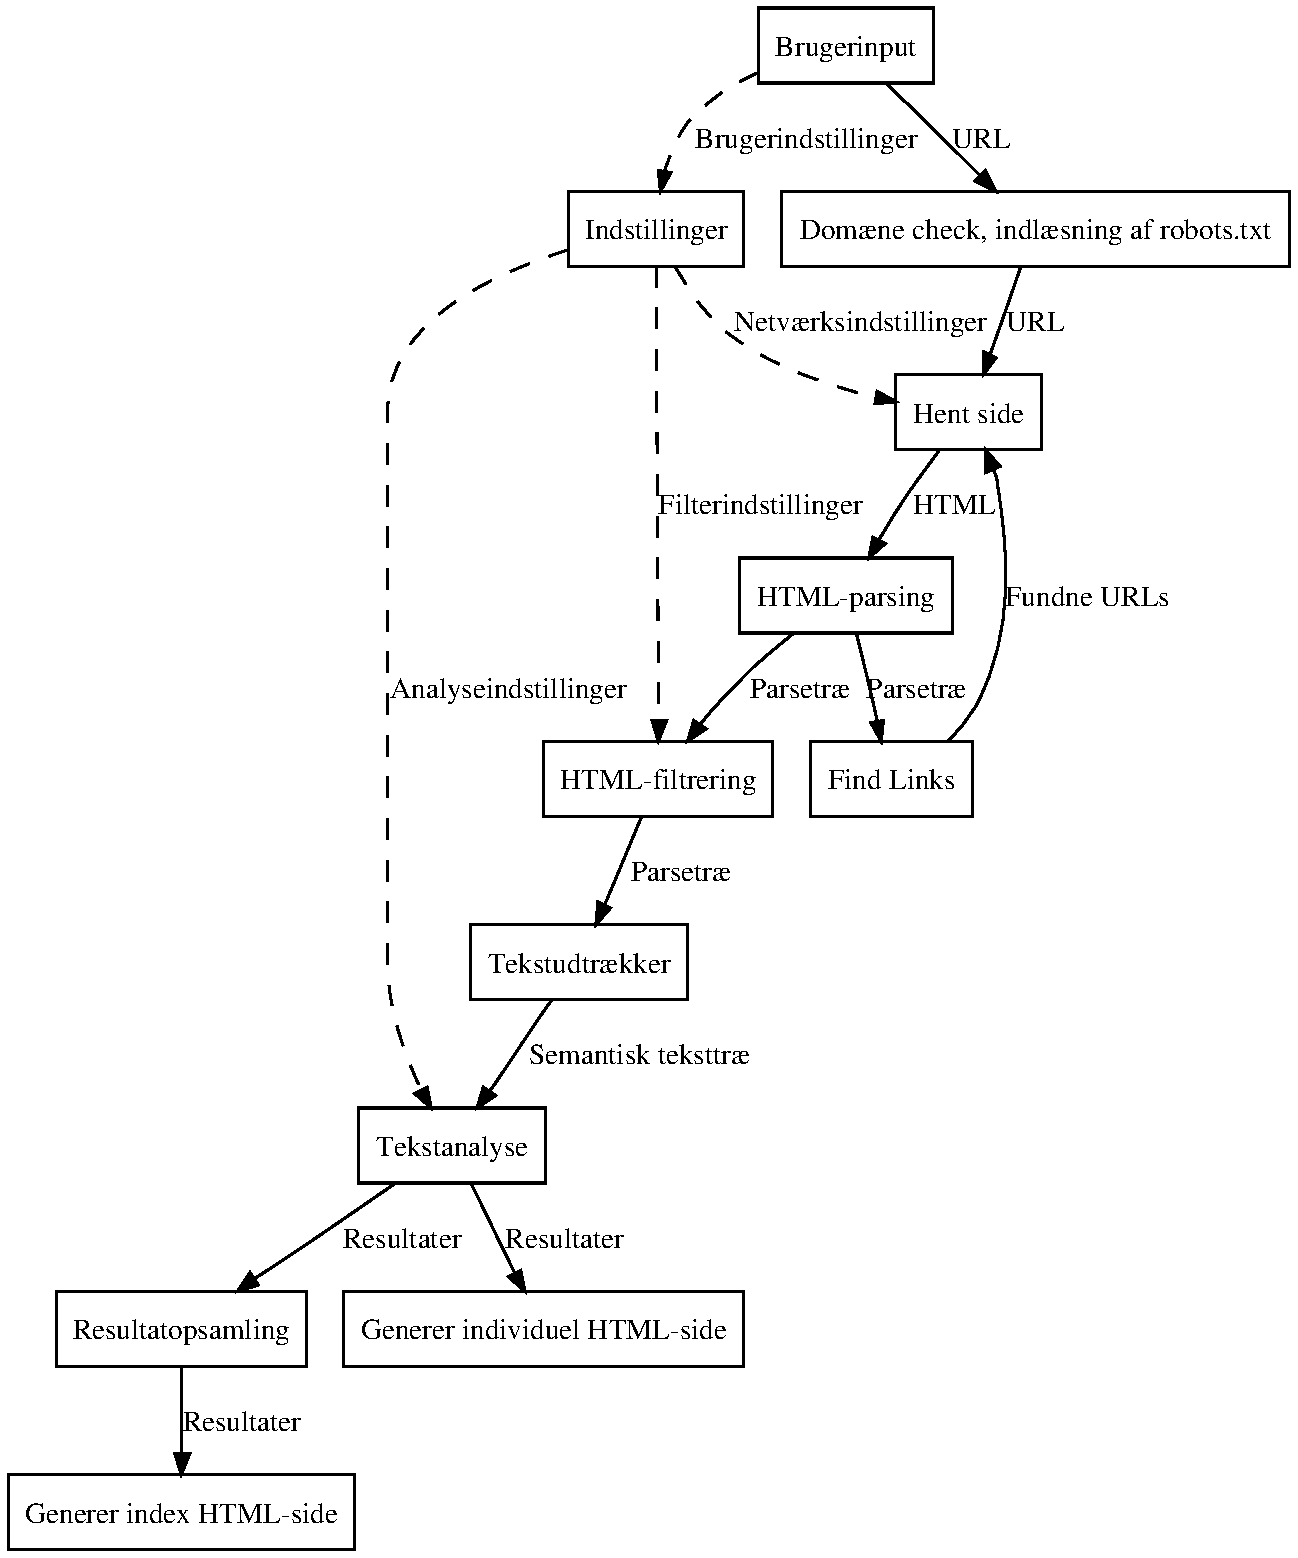
\includegraphics[width=\textwidth]{endeligtdesignill.pdf}
  \caption{Dataflow diagram}
  \label{dataflowdia}
\end{figure}

\newpage
\section{Moduler}
Vi vil nu beskrive de moduler vi har inddelt programmet i. I det
følgende henfører ``moduler'' ikke nødvendigvis til Standard ML's
modul--feature, selvom enkelte af dem er implementeret via dette
sprogkoncept.

\subsection{Brugerinput og brugervenlighed}
Dette modul skal sætte en analyse i gang ud fra de parametre brugeren
angiver. Det skal parse kommandolinjeparametrene og videregive
brugerindstillingerne til de andre moduler i programmet. Hvis
kommandolinjen er i et ugyldigt format, eller der er angivet ukendte
indstillinger, er det også dette moduls ansvar at informere brugeren
om fejlen og afslutte programmet.

\subsubsection{Brugervenlighed}
For at gøre programmet let at bruge, er det vigtigt at de
indstillinger man kan angive er lette at huske for brugeren. En bruger
vil hurtigt blive træt af at skulle slå op i manualen hver gang
programmet skal bruges. Når man starter programmet er der én
indstilling man \textit{altid} vil skulle angive --- startadressen for
analysen. Denne indstilling skal, som den eneste, ikke angives med et
specielt præfiks, fordi det alligevel altid er nødvendigt at give den
med. De andre indstillinger angives med et præfiks f.eks. \texttt{--l}
for angivelsen af sprog. Måden disse indstillinger angives, er valgt
ud fra at det skal være let at sætte deres navn/præfiks i forbindelse
med deres betydning. Eksempelvis kan man angive hvor den maksimale
dybde for analysen med indstillingen \texttt{--d}, hvor \textit{d}'et
står for \textit{depth}. Udover at det skal være let at huske
sammenhængen mellem betydning og navn, så skal tvetydigheder helst
undgås. Tvetydigheder kan gøre at brugeren husker forkert og føler det
nødvendigt at slå op i manualen. Når flere indstillinger kunne have
samme navn, har vi valgt at bruge et længere navn for at undgå disse
tvetydigheder. F.eks. er der to indstillinger der begge kan angive at
noget af dokumentet skal ignoreres i analysen, disse indstillingers
navne er \texttt{--ignore--tag} og \texttt{--ignore--id}.

\subsection{Indstillinger}
Da de brugerleverede indstillinger skal kunne tilgås fra vidt spredte
dele af programmet har vi fundet det bedst at lagre disse på et
centralt, løst koblet sted, i modsætning til programmets egentligt
arbejds--data, der i højere grad fører data rundt gennem tæt koblede
moduler og typestærke interfaces. Dette sikrer også at det er let at
tilføje nye indstillingsmuligheder --- idet der kun skal ændres i den
kode der rent faktisk udnytter den nye indstillingsmulighed --- hvor
ændringer i det primære dataflow kan resultere i en kaskade af
ændringer over det meste af programmet. Den uafhængige plads som
indstillings--informationen har i forhold til det primære dataflow
ville dog ikke være nær så passende til den primære data, idet det
ville gøre det sværere at kontrollere hvor og hvornår den blev ændret,
og ville svække muligheden for at garantere den sekventielt løbende
raffinering af arbejdsdata som programmet er bygget op omkring.

\subsubsection{Krav}
Dette modul gør det --- sammen med Brugerinput--modulet --- muligt at
opfylde krav 4 vedr. konfiguration af analyse.

\subsection{Domæne check, indlæsning af robots.txt}
Dette modul skal tjekke om det domæne brugeren har angivet kan tilgås
og give en fejlmeddelelse hvis det ikke er tilfældet. Hvis brugeren
har angivet det skal det undersøges om der er en
\textit{robots.txt}--fil (en standard, der gør det muligt for websteder
at bede søgemaskiner og andre robotter om at lade være med at besøge
dele af siden) \footnote{\url{http://www.robotstxt.org/}} på serveren
og hvis det er tilfældet så skal den parses. Informationerne i
\textit{robots.txt} skal gøres tilgængeligt for \textit{Hent
  side}--modulet, så det kan se hvilke dele af webstedet det må crawle.

\subsubsection{Krav}
Dette modul gør at vi kan opfylde første halvdel krav 1.2
\textit{``Programmet skal respektere eventuelle robots.txt filer. Det
  skal være muligt at slå dette fra.''}.

\subsection{Hent Side}
\label{hentside}
Hent side modulet skal kunne hente en side fra en webserver via
HTTP--protokollen. Da vores behov er små og vi ikke har for meget tid
vil vi bruge et eksternt produceret
HTTP--modul\footnote{\url{http://www.diku.dk/undervisning/2000e/dat0/filer200001/K1/brevkasse.html}},
modificeret til vores behov. Det er også dette moduls job at tjekke om
den indlæste \textit{robots.txt} tillader at vi må crawle siden, da dette skal
tjekkes hver gang der skal hentes en side.

Når en side er analyseret en gang, så skal den ikke analyseres igen,
hvis det skete ville programmet kunne gå i en ikke terminerende
tilstand hvis 2 sider linker til hinanden (forudsat at der ikke er
nogen dybdebegrænsning). For at undgå dette skal adressen til de
allerede besøgte sider gemmes, så det kan tjekkes at man ikke besøger
samme side igen.

\subsection{HTML--Parsing}
\label{htmlparsing}
For at kunne udtrække tekst fra en HTML--side er det nødvendigt først
at parse den. Da vi ikke har været i stand til at finde en HTML--parser
skrevet i SML har vi valgt at implementere denne selv. Resultatet af
HTML--parsingen er et ordinært parsetræ som så i senere moduler bruges
til både at danne et mere højniveau--træ over teksten, og til at finde
links til andre sider som skal hentes.

Parseren er, for at lette implementationen, opdelt i to primære dele ---
en lexer, der opdeler den indkommende sekvens af tegn i en liste af
leksikalske enheder uden nærmere struktur, og en egentlig parser, som
omdanner listen af de leksikale enheder til et struktureret
parsetræ. Lexeren er specificeret med en SML--signatur, men det er ikke
hensigten at denne bruges af andet end parser--modulet, og resten af
programmet vil ikke være påvirket af parsertrinnets toparts--opdeling.

De leksikale enheder produceret af lexeren vil være af tre forskellige
typer --- begyndelsestags, afslutningstags og tekstelementer. De to
tag--typer vil indeholde information om navnet på det relevante tag,
samt en liste indeholdende attribut/værdi--tupler. Tekstelementer vil
indeholde information om den sekvens af tegn de repræsenterer.

Det af parseren producerede parsetræ består af knuder, repræsenterende
tags, og blade, repræsenterende tekst. En knude kan have nul eller
flere undergrene der angiver de HTML--elementer der findes mellem
start-- og slut--tagget (nul undergrene kunne f.eks. være et
``\texttt{<br />}''--element), hvor hver undergren igen kan være enten
en knude eller et blad. Undergrenene skal være ordnede i samme
rækkefølge som deres optræden i det oprindelige HTML--dokument. En
knude indeholder information om hvilket tag den repræsenterer, samt
eventuelle HTML--attributter tagget har.

For eksempel vil HTML--dokumentet på figur \ref{htmldoc1} give et
parsetræ, som det illustreret på figur \ref{parsetree}. På figuren er
børnene arrangeret så det første barn står længst til venstre og det
sidste længst til højre. Hvert tag har et sæt attributter, på figuren
er indholdet af disse dog udeladt. De fleste af attributsættene er
tomme, men som det kan ses i HTML--dokumentet så har
\texttt{BLOCKQUOTE}-- og \texttt{A}--tagsne en attribut hver.
I parsetræet er der også en del mellemrums--tegn der er ikke er
medtaget for at simplificere figuren.

\begin{figure}
\begin{lstlisting}[language=HTML,
                   escapechar=\@]
<HTML>
  <HEAD><TITLE>Sidetitel</TITLE></HEAD>
  <BODY> <!-- En kommentar -->
    <P>Et afsnit med adskillige s@\ae@tninger.
      Dette er 'den anden s@\ae@tning'.</P>
    <BLOCKQUOTE lang="en">
      <A href="http://en.wikipedia.org/wiki/Hovercraft">My hovercraft</A>
      is full of eels!</BLOCKQUOTE>
  </BODY>
</HTML>
\end{lstlisting}

  \caption{Eksempel HTML--dokument.}
  \label{htmldoc1}
\end{figure}

\begin{figure}
  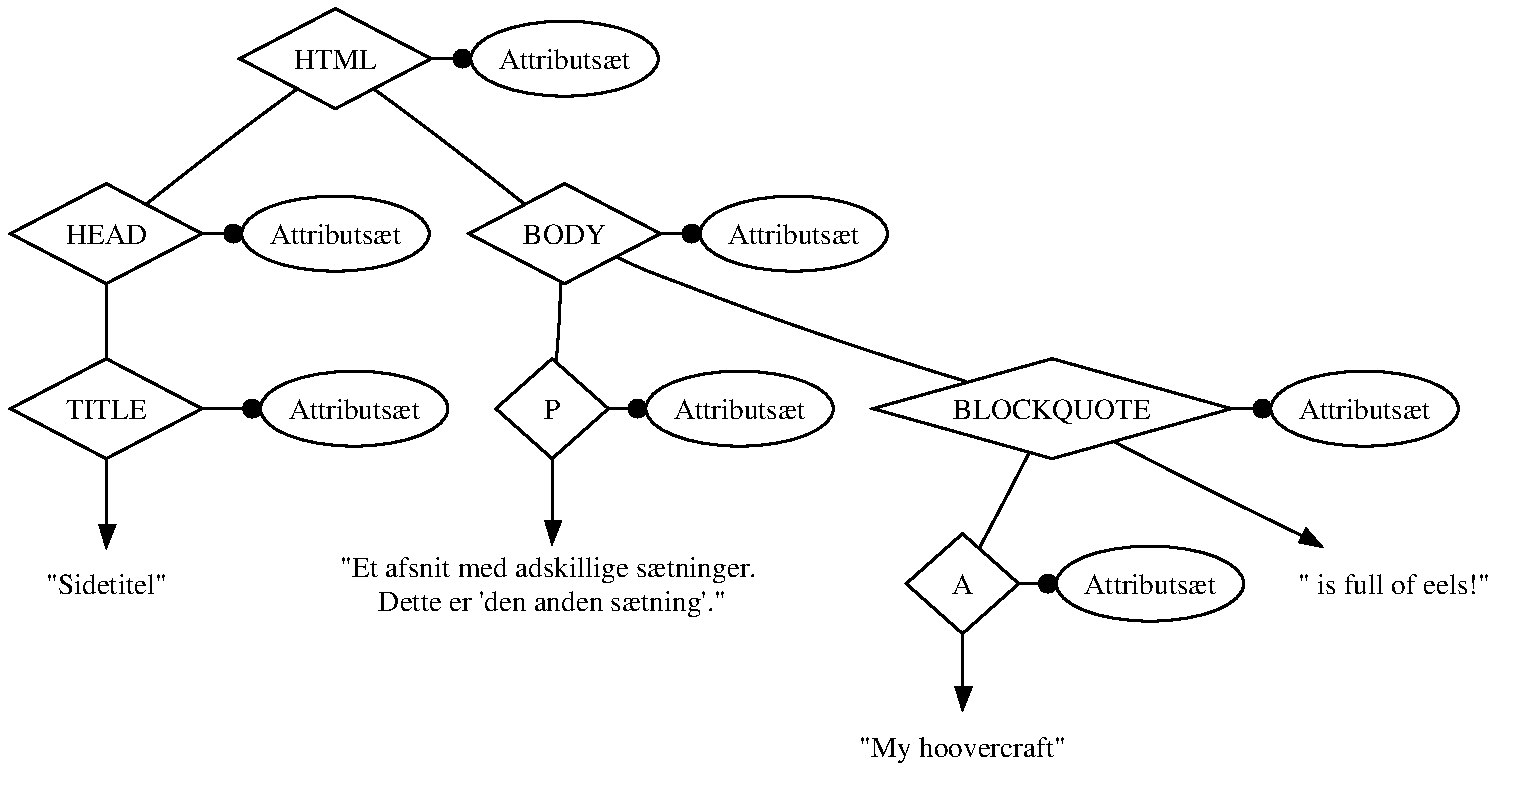
\includegraphics[width=\textwidth]{parsetree.pdf}
  \caption{Parsetræ for HTML--dokumentet på figur \ref{htmldoc1}.}
  \label{parsetree}
\end{figure}

En beskrivelse af implementationen af HTML--parseren er at finde i
sektion \ref{htmlparserimpl}.

\subsection{Find links}
Dette modul skal ud fra HTML--parsetræet genereret af HTML--parseren,
lave en liste af de links som linker til andre sider på samme domæne.
Det skal derefter bede om at disse sider bliver hentet, parset og
analyseret, og undersøge links på de nyhentede sider --- en rekursiv
proces der løber indtil alle tilgængelige sider er blevet analyseret.

For at finde linksene skal alle \texttt{a}--tags findes --- deres
\texttt{href} attribut angiver så det link der peges på. De adresser
man finder kan være relative til den nuværende side. Den absolutte
adresse til den nuværende side skal derfor kombineres med den relative
sti fra linket for at forme linkets absolutte sti. Det er dog ikke
altid den nuværende sides absolutte sti som adresser skal være
relative til, man kan angive en anden sti som de skal være relative
til med \texttt{base}--tagget. Da \texttt{a}--tags også bruges til andet 
end links til almindelige htmlsider, sørger vi for at filtrere dette fra. 
Dette kunne f.eks. være links til mails \texttt{mailto:} eller javascript
funktioner \texttt{javascript:}

Det er ikke kun \texttt{a} der skal undersøges, hvis et HTML--dokument
benytter sig af rammer (frames), så skal deres start--adresser også
findes. Der er også andre tags der tillader at man specificerer
adresser til forklaringer ol, disse skal der også tages hån om.
\label{cyklus}
  På dataflowdiagrammet (figur \ref{dataflowdia}) går kun en enkelt pil fra
``Find links''--modulet til ``Hent side''--modulet. Reelt bliver denne pil fulgt
for hvert eneste
fundet link som ikke allerede er blevet besøgt --- resultatet bliver at
cyklussen i diagrammet fungerer som programmets primære loop der
henter og analyserer links, indtil der ikke kan findes flere indenfor
den angivne maksimaldybde.

\subsubsection{Krav}
At vi kan finde links på en hjemmeside gør at vi kan opfylde krav 1
der siger at man skal kunne foretage en analyse af et helt websted.

\subsection{HTML--filtrering}
For at gøre det muligt at angive at nogle dele af en hjemmeside ikke
skal analyseres er det nødvendigt med et modul der kan frasortere de
ønskede elementer fra siden. Ud fra brugerens indstillinger skal dette
modul kunne frasortere dele af en HTML--side. Dette kan f.eks. bruges
til at frasortere menuer, brugerkommentarer og andet tekst som vil
kunne påvirke analysen, på en måde så resultatet bliver
misvisende. Beregningen af læsbarhedsindekset kan eksempelvis blive
påvirket af at der i menuer ofte er en stor andel lange ord.

\subsubsection{Krav}
HTML--filtreringen er medvirkende til at vi kan opfylde krav 4
vedr. konfiguration af analysen.

\subsection{Tekstudtrækker}
\label{tekstudtraekkerdesign}
Når et HTML--dokument er parset kan vi udtage teksten, det er dette
moduls job at læse parsetræet for et HTML--dokument og omdanne det til
afsnit, sætninger, overskrifter osv, som \textit{Tekstanalyse}--modulet
kan analysere. Udover at opdele teksten skal de enkelte tekstpassagers
semantiske betydning bibeholdes.

\begin{figure}
  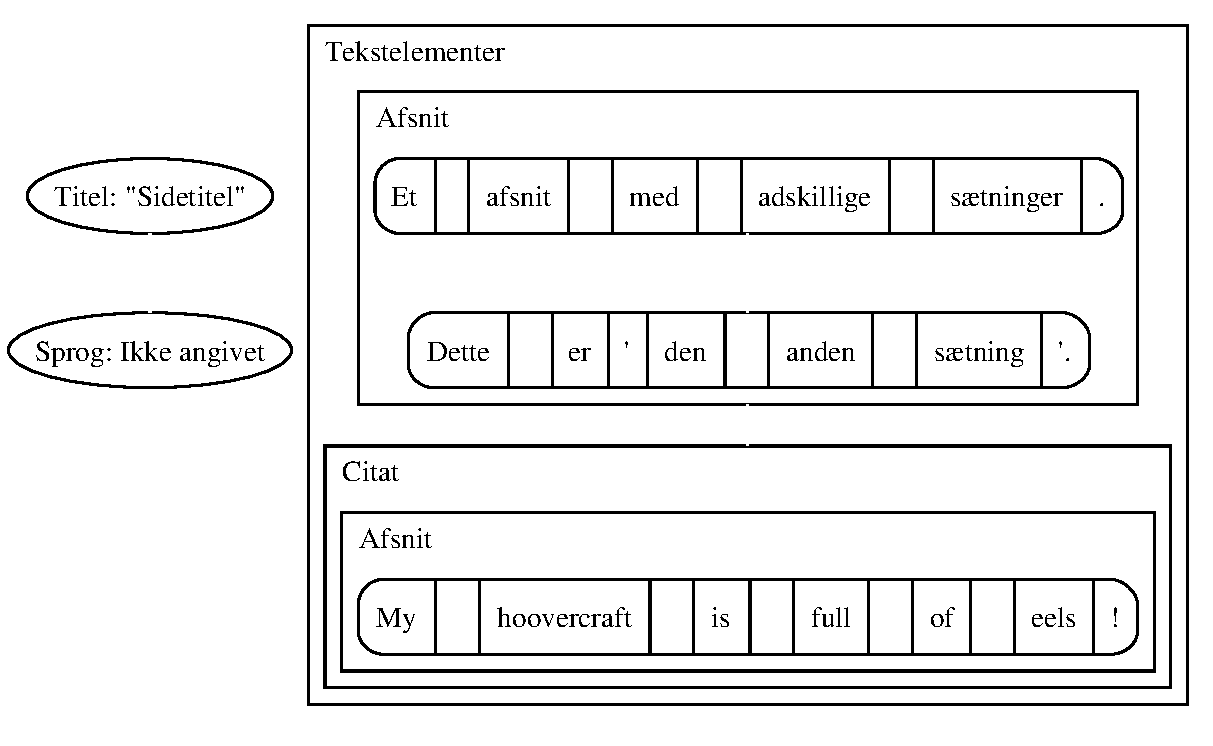
\includegraphics[width=\textwidth]{documentill.pdf}
  \caption{Resulterende dokument--struktur for parsetræet på figur
    \ref{parsetree}}
  \label{dokument}
\end{figure}

På figur \ref{dokument} er vist et eksempel på den resulterende
datastruktur. Dokumentet består af en titel, et sprog og en liste af
tekstelementer. Et tekstelement er enten en overskrift, et citat eller
et afsnit. Afsnittene er de mest interessante, da overskrifter og
citater i sig selv blot består af en liste afsnit. I HTML angives
afsnit med \texttt{P}--tagget, men der er også en række andre tags der
adskiller teksten i afsnit, f.eks. startes der et nyt afsnit efter et
billede, en tabel, faktisk sker det ved alle tags der er
``block--elementer''. Et afsnit består af en række sætninger og en
række ``ekstra'' sætninger som er den tekst der ikke umiddelbart
optræder på HTML--siden, men som alligevel er interessant --- såsom
\texttt{title} og \texttt{alt}--tekst for links og billeder (disse er
ikke vist på figuren). Sætningerne er opdelt i ord og punktuering
(tegnsætning, mellemrum mv.) og hver sætning slutter ved et eller
flere punktummer, spørgsmålstegn eller udråbstegn. Hvert ord har
semantisk information fra HTML'en tilknyttet, som f.eks. information
om hvorvidt ordet er en forkortelse, eller oprindeligt har været inde
i et \texttt{em}--tag.

For ikke at låse programmet fuldstændig fast til HTML er dette modul
delt i to delmoduler. Det ene modul (den egentlige tekstudtrækker)
kender til selve HTML--formatet og omdanner det til en mere generisk
datastruktur der symboliserer et dokument. Denne datastruktur
indeholder information om tekstens inddeling i afsnit, overskrifter,
citater mm. Datastrukturen viderebehandles af det andet delmodul
sætnings--opdeleren, som udfører de
beregninger der er ens for
alle dokumenter. Dette inkluderer adskillelse af ord og punktuering
(mellemrum, tegnsætning mv.) og opdeling i sætninger.  Det første
delmodul kan på denne måde let udvides så det også kan håndtere andre
dokumentformater.

\subsubsection{Krav}
Tekstudtrækkeren giver os muligeheden for at opfylde krav 3 og alle
dets underkrav, ved at hente den semantiske information fra
HTML--tags.

\subsection{Tekstanalyse}
\label{tekstanalysedesign}
Her skal de egentlige analyser foretages, modulet får teksten fra
\textit{Tekstudtrækkeren} og udfører de af brugeren valgte
tekstanalyser.

Til beregning af både lixtal og Flesh Reading Ease skal bruges
informationer om bl.a. antal ord og antal sætninger. Det vil resultere
i dobbeltarbejde hvis flere analyser beregner disse tal, for at
afhjælpe dette vil vi lave en forudgående indsamling af informationer
om teksten, der kan være relevante for flere af analyserne. Dette vil
også lette arbejdet med evt. implementation af yderligere
tekstanalyser, da det i princippet kun er den matematiske formel der
skal indtastes, medmindre meget specifikke informationer ønskes
(f.eks. ``Hvor mange ord er der med 3 stavelser eller færre?'').

Uddata fra tekstanalysemodulet er en datastruktur der meget ligner
input, men som i stedet for semantisk information har fået tilknyttet
læsesværhedsgrad--data til de leksikale enheder (afsnit, sætninger og
ord).

Det er også i analysemodulet at ord stavekontrolleres baseret på deres
angivne sprog, og får tilknyttet en værdi der angiver om de er korrekt
stavet eller ej. Til at foretage selve stavekontrollen vil vi bruge
GNU Aspell\footnote{\url{http://aspell.net/}}. Vi mener ikke det er et
urimeligt krav til brugerens system at GNU Aspell skal være
installeret, da det er et relativt almindeligt program på
GNU/Linux-systemer (vor målplatform). For at gøre det muligt senere at
skifte til en anden type stavekontrol, er det bedst at denne
funktionalitet er adskilt så meget fra resten af programmet som
muligt. Vi vil derfor indkapsle stavekontrollen i sit eget delmodul,
som det egentlige tekstanalyse--modul kan forespørge.

\subsubsection{Krav}
Dette modul gør at vi kan opfylde krav 2 (vedr. analysemetoder) og
alle dets underkrav.

\subsection{Generer individuelle HTML--sider}
Dette modul skal lave de HTML--filer der skal præsentere
analyseresultaterne for brugeren. Givet analyse resultaterne for en
enkelt side skal det generere en HTML side. HTML--siden vil få et
deterministisk navn baseret på HTML--filens navn og placering på
webstedet, således at der kan skabes links til den genererede HTML--fil
fra analyseindekset. Til at generere HTML'en bruger vi et modul
baseret på Msp (ML Serverpages), dette er en del af Moscow ML's
standardbibliotek\footnote{\url{http://www.dina.kvl.dk/~sestoft/mosmllib/Msp.html}}.

\subsubsection{Krav}
Dette modul er medvirkende til at vi kan opfylde krav 6, der
bl.a. siger at programmet skal generere HTML--filer der viser
resultatet.

\subsection{Resultatopsamling}
For hver side udregnes en sidesværhedsgrad som skal vises på
oversigtssiden for analyseresultatet. Dette modul skal gemme
sidesværhedsgrad for hver side, så der kan genereres en index fil når
analysen af alle undersiderne er afsluttet.

\subsection{Generer index HTML--side}
For at brugeren nemt kan få adgang til analyseresultaterne vil vi også
generere en index fil. Dette skridt er det absolut sidste der tages i
programmet, og først når alle webstedets undersider er blevet
analyseret.

\subsubsection{Krav}
Dette modul er sammen med resultatopsamleren og modulet til generering
af individuelle HTML--sider med til at opfylde krav 6.

\section{Redegørelse for designets kvaliteter}
Ved at bruge dette design vil vi kunne indfri alle de krav der er
stillet i kravspecifikationen. Som omtalt ved Tekstudtrækkeren
(sektion \ref{tekstudtraekkerdesign}) og tekstanalyse-modulet
(sektion \ref{tekstanalysedesign}) gør dette design det nemt at udvide
programmet med yderligere tekstformater og analysemetoder.

Alle modulerne kan testes automatisk. Dog er det ikke muligt at lave
en decideret unit--testing af alle modulerne, da de er så tæt koblede
som de er. Hvis man vil teste Tekstudtrækkeren skal man f.eks. bruge
et parsetræ som kun kan genereres af HTML--parseren.

Den klare opdeling i moduler som udveksler data gør det muligt at
parallelisere udviklingen, således at de enkelte moduler kan
implementeres for sig selv, uden at afhænge af en færdig
implementation af de andre moduler (deres signaturer skal dog være
lagt på plads). Hvert konceptuelt modul kan, om ikke fuldstændigt, så
til en vis grad, implementeres som en SML modulsignatur og struktur.

\chapter{Implementation}
\label{implementation}

\section{Arbejdsfordeling}

Vi forsøgte ikke at inddele implementationsarbejdet på forhånd. I
stedet meldte medlemmer af gruppen sig frivilligt til at implementere
dele af programmet når det blev relevant, og deres viden om den kode
de selv havde skrevet gjorde dem sidenhen til den naturlige
vedligeholder af den relevante del af programmet. Programmet bærer
derfor præg af at forskellige personer har arbejdet på forskellige
dele af det, men uden at grænserne mellem de forskellige
gruppemedlemmers primære områder nødvendigvis er trukket efter logiske
implementationslinjer.

Følgende tabel angiver de primære forfattere af de forskellige
kodefiler i programmet.

\begin{longtable}{l|c|c|c}
\textbf{Fil} &
\textbf{Jesper} &
\textbf{Martin} &
\textbf{Troels} \\ \hline
Load.sml & $\surd$ & $\surd$ & $\surd$ \\ \hline
Main.sml & $\surd$ & $\surd$ & $\surd$ \\ \hline
Config.(sml|sig) & $\surd$ & $\surd$ & $\surd$ \\ \hline
Robots.(sml|sig) & $\surd$ & & \\ \hline
HTMLLexer.(sml|sig) & & & $\surd$ \\ \hline
HTMLParser.(sml|sig) & & & $\surd$ \\ \hline
HTMLFilter.(sml|sig) & & $\surd$ & \\ \hline
TextExtractor.(sml|sig) & & $\surd$ & \\ \hline
Sentencifier.(sml|sig) & & $\surd$ & $\surd$ \\ \hline
TextAnalyser.(sml|sig) & & $\surd$ & \\ \hline
TextAnalysisReporter.(sml|sig) & $\surd$ & $\surd$ & $\surd$ \\ \hline
SpellChecker.(sml|sig) & & & $\surd$ \\ \hline
Util.(sml|sig) & $\surd$ & $\surd$ & $\surd$ \\ \hline
Help.(sml|sig) & $\surd$ & & \\ \hline
%webanalyzer.1 & $\surd$ & & \\ \hline
% Test.sml & $\surd$ & & \\ \hline
% Test.Robots.sml & $\surd$ & & \\ \hline
% Test.HTMLParser.sml & $\surd$ & & \\ \hline
% Test.Analyser.sml & $\surd$ & & \\ \hline
\end{longtable}

\section{Parsing af HTML}
\label{htmlparserimpl}
For korrekt at udtrække tekst, og information om teksten, fra et
websted, er det nødvendigt at kunne parse HTML, eller have en anden
måde at adskille tekst fra tags og forbinde informationen i tags til
den tekst der står under dem. I vores program valgte vi at
implementere en nogenlunde fuldgyldig HTML parser (se nedenfor for
dens begrænsninger), da vi mente at det ville være lettere at udtrække
information fra et parse--træ, end hvad søgning med f.eks. regulære
udtryk ville resultere i. Blandt andet på grund af vores begrænsede
tidsresurser var der en række krav til parseren og dens
implementation:

\begin{itemize}
\item Den skal kunne håndtere både HTML og XHTML (se sektion
  \ref{begraensning}), idet vi ikke har tid til at implementere to
  forskellige parsere. Heldigvis minder HTML og XHTML meget om
  hinanden, og XHTML-sider udnytter sjældent XML's mere avancerede
  features, så vi valgte ikke at understøtte disse.
\item Vi valgte at undlade at forsøge at håndtere indholdet af
  \texttt{script} og \texttt{style}-tags korrekt, til trods for at
  indholdet af disse kan indeholde tekst der kan forvirre
  parseren. Grundet tidsnød valgte vi at undlade at implementere denne
  håndtering, et problem der er begrænset i omfang, idet størsteparten
  af moderne sider specificerer eksterne scripts og
  \textit{CSS--stylesheets}, hvis indhold altså ikke ligger direkte i
  HTML-dokumentet, og som derfor ikke kan forvirre
  parseren. \textbf{Dette er en afvigelse i forhold til vores
  kravspecifikation}. Det kan også nævnes at vi under alle
  omstændigheder ikke have tænkt os at foretage os noget med
  indlejrede scripts eller stylesheets (se sektion
  \ref{begraensning}).
\item Vi garanterer kun at vi kan håndtere korrekt HTML, men vi
  ønskede også at parseren skulle kunne håndtere visse typiske fejl,
  såsom at glemme at lukke tags.
\end{itemize}

Idet ingen i gruppen havde erfaring med brug af
parser--generatorer\footnote{f.eks. SML-YACC og SML-Lex.}
blev det vurderet at det mest effektive ville være at skrive
HTML--parseren i hånden. Af simplicitetshensyn valgte vi at dele den
op i to dele --- en lexer der behandler bogstaver direkte, og en
parser, der behandler de leksikalske enheder der produceres af lexeren
(se vores design, sektion \ref{htmlparsing}).

\subsection{HTML--lexer}
\label{htmllexerimpl}
Lexer--algoritmen er baseret på en simpel tilstandmaskine. Overordnet
findes der en funktion, \texttt{lexer}, der tager et tegn og en
\textit{tilstands--værdi} som argumenter, og returnerer en ny
tilstandsværdi. Funktionen bliver gentagne gange kaldt med tegnene fra
HTML-dokumentet, samt den tilstandsværdi som blev returneret ved
sidste kald, indtil der ikke er flere tegn tilbage i
HTML-dokumentet. En af disse tilstandsværdier er speciel og angiver at
lexeren er færdig med at lexe en leksikalsk enhed. Den producerede
leksikalske enhed er en del af denne tilstandsværdi, og ``samles op''
af den omkringliggende kode, hvorefter \texttt{lexer}--funktionen
kaldes igen med en særligt ``ny start'' tilstands--værdi, der også
bruges ved første kald til funktionen. De andre tilstands--værdier
indeholder information om hvor langt lexeren er nået med at lexe en
given leksikalsk enhed, og deres indhold undersøges ikke af den
omkringliggende kode, men bruges udelukkende til at foretage et nyt
kald til \texttt{lexer}. Lexeren producerer tre forskellige typer af
leksikalske enheder: Start--tags, slut--tags og tekst, der ikke er et
tag. De leksikalske enheder for tags indeholder også information om de
attributter de relevante tags har, noget man normalt ville placere i
selve parser--delen. På den måde producerer vores HTML--lexer relativt
detaljeret leksikalske enheder i forhold til hvad man normalt ville
forvente af en lexer.

Funktionen \texttt{lexer} er implementeret som en stor
mønstergenkendende (\textit{pattern--matching}) funktion der baseret
på lexertilstanden, og det leverede tegn, genererer en ny
lexertilstand. Funktionen er deklarativt implementeret, idet der
næsten ingen logik er i funktionen, med undtagelse af
mønstergenkendelsen. Dette resulterer i at funktionen ganske vist
fylder mange linjer, men til gengæld nærmest kan læses som en tabel
over lexing af HTML, noget der gør det relativt nemt at bedømme hvad
den gør, og som har resulteret i at den gennem programmets udvikling
har haft meget få fejl i forhold til resten af koden. Lexeren er
implementeret således at den kan fungere med vilkårligt stort input,
så længe der er tilstrækkeligt med hukommelse. Dette fandt vi
nødvendigt, idet et HTML-dokument let kan indeholde flere tusinde
tegn.

\begin{figure}[h]
  \begin{tabular}{lll}
\textbf{Inddata} &
\textbf{Lexertilstand} \\

$\blacksquare$<a href=``foo''> & New \\
\hspace*{10pt}$\blacksquare$a href=``foo''> & LexingTag \\
\hspace*{10pt}<$\blacksquare$ href=``foo''> & LexingTagName \\
\hspace*{10pt}<a$\blacksquare$href=``foo''> & LexingAttributes \\
\hspace*{10pt}<a $\blacksquare$ref=``foo''> & LexingAttributeName \\
\hspace*{10pt}<a h$\blacksquare$ef=``foo''> & LexingAttributeName \\
\hspace*{10pt}<a hr$\blacksquare$f=``foo''> & LexingAttributeName \\
\hspace*{10pt}<a hre$\blacksquare$=``foo''> & LexingAttributeName \\
\hspace*{10pt}<a href$\blacksquare$``foo''> & LexingAttributeValueStart \\
\hspace*{10pt}<a href=``$\blacksquare$oo''> & LexingAttributeValue \\
\hspace*{10pt}<a href=``f$\blacksquare$o''> & LexingAttributeValue \\
\hspace*{10pt}<a href=``fo$\blacksquare$''> & LexingAttributeValue \\
\hspace*{10pt}<a href=``foo''$\blacksquare$ & LexingAttributes \\
\hspace*{10pt}<a href=``foo''>$\blacksquare$ & Done \\
\end{tabular}
  \caption{Eksempel af lexeme returneret af lexeren ud fra givet et tegn
i indput. Den sorte firkant indikerer det tegn som lexeren behandler}
  \label{ekslexeroutput}
\end{figure}

\subsection{HTML--parser}

Grundet HTML--lexerens detaljerede output (se sektion
\ref{htmllexerimpl}) er parseren relativt simpel --- dens opgave er at
finde ud af hvilke børn et tag har (se sektion \ref{htmlparsing}), og
sætte det sammen til et træ.

Den overordnede algoritme er som følger: Parseren ser en leksikalsk
enhed. Er denne ikke et tag, gemmes den, og næste leksikalsk enhed
analyseres. Hvis enheden dog er et tag findes alle leksikalske enheder
op til et matchende slut--tag, og disse indsættes som børne--elementer
til det fundne tag. Parsingen går videre med den leksikalske enhed
efter slut--tagget. Børne--elementerne parses naturligvis også, så de
også får træstrukturen.

Parseren er, i modsætning til lexeren, \textit{ikke} skrevet således
at den kan håndtere arbitrært stort input. Den primære parserfunktion
er en rekursiv, men ikke hale--rekursiv, funktion som kalder sig selv
for at finde både børne--elementer og efterfølgende elementer. Den er
derfor begrænset i hvor ``dybe'' og ``lange'' dokumenter den kan
håndtere, hvor grænsen er sat ved SML--implementationens maksimale
kaldstak--dybde. Da parseren dog opererer på leksikalske enheder, som
der ofte er relativt få af i forhold til tegn i dokumentet, opfatter
vi dog ikke dette som et problem i praksis. Det er mere sandsynligt at
computeren løber tør for hukommelse under indlæsning af et for stort
HTML--dokument end at parseren laver stakoverløb.

\section{Robots.txt}
\label{robots} 

\textit{The robots exclusion standard} eller \textit{Robots Exclusion Protocol}
er en meget simpel standard som dog ikke er godkendt af nogle officielle
organisationer, men udtrykker en enighed mellem
internet robot\footnote{``webrobots'',
``spiders'' og andre former for internet crawlere} forfattere og andre med
interesse inden for internet robotter. Da det ikke er en officel standard skal
det blot ses som almene retningslinjer.

\subsection{Forklaring, opbygning og syntaks af robots.txt}
Filens format\footnote{\url{http://www.robotstxt.org/wc/norobots.html\#format}}
består af en eller flere statements separeret af et eller flere tomme linjer.
Hver linje indeholder statements på formen:\\
``<field>:<optionalspace><value><optionalspace>'' hvoraf \texttt{field} er case
insensitive og ``\#'' indikerer at det efterfølgende mellemrum (hvis der er et)
og alt til og med linjens afslutning skal ignoreres (fortolkes som kommentarer).

Filen(Se figur \ref{eksrobotstxtfile} for eksempel på en robots.txt fil) starter
med en eller flere \texttt{user-agent}\footnote{Værdien af dette
statement er navnet for den robot som der angives adgangs politik for}
statements efter fulgt af en eller flere \texttt{disallow}\footnote{Værdien af
dette statement angiver en relativ \texttt{URL} som ikke må crawles. Dette kan
være en full sti eller en del af en sti, hvilket angiver at alle \texttt{URL}s
som prefixes af dette ikke må crawles.} statements\footnote{Der er foreslået
udvidelser til standarden som udervider funktionaliteten med flere statements,
se: \url{http://en.wikipedia.org/wiki/Robots.txt}} 
Ikke genkendte start statements i filen bliver ignoreret.

\begin{figure}[h]
\begin{lstlisting}[language=csh,
                   escapechar=\@]
  User-agent: BadBot
  Disallow: /
  # Kommentarer forekommer efter "#" symbolet ved linje start eller
  User-agent: *                          # efter et statement
  Disallow: /directory/file.html
  Disallow: /private 
  Request-rate: 2/10    # Medf@\o@rer 10sek/2sider = 5sek crawl delay
\end{lstlisting}

  \caption{Eksempel på en robots.txt fil}
  \label{eksrobotstxtfile}
\end{figure}


\subsection{Implementation}

For at kunne overholde en eventuel robots.txt, Hentes og parses denne fil.
Parseren leder efter alle user-agent værdier som matcher
programmets egen\footnote{Defineret i Config modulet} og ``*''. Herefter
parses alle de fundne statements.

Parseren kan forstå det almindelige \texttt{disallow} statement men
ydermere har vi også implementeret \texttt{request-rate} fra den udvidede
standard\footnote{\url{http://en.wikipedia.org/wiki/Robots.txt}} og
\texttt{crawl-delay} som ikke er en del af den udvidede standard men blot et
forslag af mange som kompliment til \texttt{request-rate}'s besynderlige
syntaks. 

Vi har explicit valgt ikke at implementere andre statements fra den
udvidede standard da disse ikke har nogen praktisk betydning for vores
program.

Når \texttt{robots.txt} er parset kan man query Robots modulet om en given
relativ URL må crawles eller ej. Dette gøres ved at løbe listen igennem
og se om der findes et match der prefixer den relative url.

Når parseren finder et \texttt{crawl-delay} statement eller 
\texttt{request-rate}\footnote{Værdien af \texttt{request-rate}
angives som \#SIDER/\#SEKUNDER og laves derfor om og udregnes som
$\dfrac{sekunder}{sider}$ så der fås et \#delay pr side} statement
gemmes det angivne tids værdi i Config modulet.

\section{Dybde håndtering}

Når sider bliver analyseret og links fundet, gemmes disse med den
pågældende dybde de ligger i. Når der herefter skal trækkes ud fra
denne liste bruges bredde--først søgning. Da hvis man havde brugt
dybde--først søgning på figur \ref{depthtree} og maksimal crawl--dybde
på 2, ville man ende med at startside, underside X, underside Y blev
analyseret, da hovedsiden også linker direkte til underside Y bør
underside Z også komme med i analysen da den ved denne vej har dybde
2, men dette sker ikke da underside Y allerede er analyseret og bliver
ignoreret ved alle fremtidig referencer på nær den første, grundet
vores liste over allerede analyserede sider (se sektion \ref{hentside}).
På baggrund af dette bruges bredde--først søgning hvorved dette problem
ikke opstår, da bredde--først søgning starter med at analysere startsiden,
underside X, underside y, underside y (linket fra underside x, men bliver
ignoreret grundet den allerede er besøg) og underside z.

\begin{figure}[h]
  \centering
  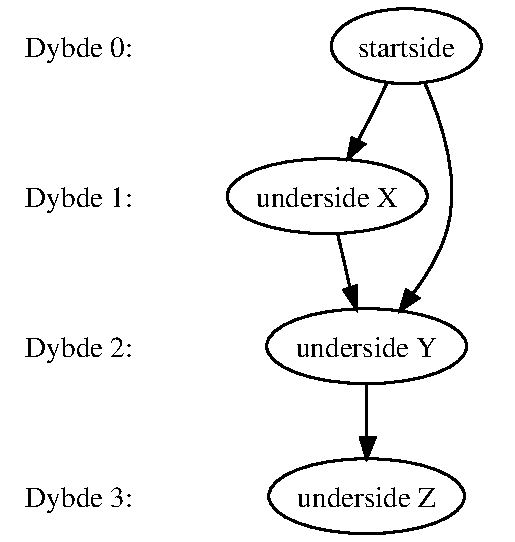
\includegraphics[width=0.5\textwidth]{depthtreeill.pdf}
  \caption{Eksempel på dybden af links på et simpelt websted}
  \label{depthtree}
\end{figure}

\section{Tekstudtrækker}
Tekstudtrækkerens job er som beskrevet i designet (sektion
\ref{tekstudtraekkerdesign}), at omdanne HTML--dokumenter til en
generisk dokumentstruktur som tekstanalyse--modulet kan
analysere. Dette inkluderer opdeling i afsnit, overskrift og citater,
samt opdeling af afsnit i ord og sætninger.

HTML--dokumenter har ofte dybe indlejringer i form af \texttt{div}--
eller \texttt{table}--tags som bliver brugt til at opsætte hjemmesiden
som ønsket. I almindelige dokumenter er vi dog ikke interesserede i
denne slags indlejring. Tekstudtrækkerens job består således også i at
fladgøre det parsetræ som den får leveret. I vores implementering af
fladgøringen gennemgår vi træet ved at gennemgå parsetræet med
\textit{inorder tree walk}, på vejen ned igennem træet opsamler vi de
semantiske informationer (f.eks. om sprog) som er angivet, sådan at vi
kan klistre dem på det tekst vi møder. Når vi møder et tekstelement
indsætter vi teksten sammen med de, på daværende tidspunkt, opsamlede
informationer. Når vi møder et tag der kan adskille teksten i afsnit,
så indsætter vi et symboler der indikerer \textit{``nyt afsnit''} før
og efter indholdet af det pågældende tag (der rekursivt er
fladgjort). Efter fladgøringen har vi så en liste hvor teksten har
fået klistret semantisk informationer på og hvor der er symboler hver
gang der starter et nyt afsnit. Som omtalt ovenfor bliver tabeller og
\texttt{div}--tags ofte brugt til at lave layout med, og mange steder
i forbindelse med den slags tags vil der derfor blive indsat en stor
dosis \textit{``nyt afsnit''}--symboler. For at undgå tomme afsnit
fjerner vi flere på hinanden følgende \textit{``nyt
  afsnit''}--symboler og erstatter dem med et enkelt.

\subsection{Ord og Sætningsopdeling}
Efter HTML--dokumentet er omformet til en mere generisk
dokument--struktur, skal teksten opdeles i ord og sætninger. Intuitivt
ville det måske være mest naturligt først at opdele teksten i
sætninger og derefter i ord, da man på den måde gradvist opdeler i
mindre og mindre dele. Sætninger opdeles primært af punktummer, men
punktummer bliver også brugt i forbindelse med forkortelser og hvis
man bare opdelte teksten ved alle punktummer ville man kunne komme til
at dele en sætning midt i en forkortelse. Vi har i stedet adskilt
teksten i ord og punktuering til at starte med og ved identificeringen
af ord har vi implementeret en simpel
forkortelsesgenkendelse (se nedenfor). Derefter opdeler vi listen af ord i
sætninger ved alle følger af punktuering der indeholder en
sætningsafslutter (punktum, spørgsmålstegn og udråbstegn).

Den omtalte forkortelsesgenkendelses mekanisme er meget simpel, hvis
bogstavet der kommer efter et punktum er et lillebogstav, så antager
vi at punktummet afslutter en forkortelse, det samme sker hvis vi
finder et bogstav midt i et ord (dvs. uden mellemrum efter
punktummet). Derudover antager vi at enkeltstående store bogstaver
efterflugt af et punktum er et initial. Eksempelvis afslutter
punktummet i ``H. Hansen'' ikke en sætning. Disse antagelser betyder
dog ikke at vi altid opdeler sætninger korrekt, faktisk kan der opstå
andre fejl pga. forkortelseshåndteringen. Eksempelvis vil disse 2
sætninger ikke blive adskilt: \textit{``Hun stemte på liste O. Det var jo en
ren fadæse!''}.

\section{Tekstanalyse}
\label{tekstanalyse}

\fixme{Skriv herremeget her.}

Udover selve brødteksten indeholder hjemmesider også en masse ``støj''
i form a navigationstekst, og andre minisætninger rundt omkring. Disse
er alt for små til at fungere ordentligt med analysemetoderne og
resulterer i at der optræder forstyrrende information i
analyseresultatet. Især er enkeltstående lange ord et problem ---
ordet ``rejseomkostninger'' stående alene vil, når det bliver
analyseret, ende med et resultat der er helt hen i vejret, og selvom
det ikke har stor betydning for vurderingen af siden som helhed,
skaber støj på analyseresultat--siden. At løse det generelle problem,
at filtrere ``uinteressant'' sidetekst fra, har vi ikke løst, idet vi
vurderede det som for svært. I stedet har vi indsat en nødløsning,
hvori afsnit der har en FRE værdi på under -50 og over 200 (normalt
siger man at skalaen går fra 0 til 100 for almindelig tekst) filtreres
fra det resultat der vises til brugeren, såfremt disse afsnit ikke
indeholder stavefejl\footnote{Grunden til at elementerne ikke bliver
  filtreret fra er fordi det stadig er relavant at vise stavefejl
  iht. analysen. Se kravspecifikationen, krav 2.3 Stavekontrol}. Dette
gøres for ikke at forstyrre brugeren med dårligere resultater.

\section{Stavekontrol}
\label{spellchecker}


Tekstanalyse strukturen foretager en stavekontrol af hvert ord den
møder. Til at foretage stavekontrollen har vi implementeret en
struktur \texttt{SpellChecker} der med funktionerne
\texttt{spellCheckWord} og \texttt{spellCheckWords} kan angive om ord
er stavet korrekt. Til at gøre dette bruger vi GNU Aspell, dette er
væsentligt nemmere end at implementere et nyt stavekontrolsystem i selve
vores program. SpellChecker--strukturen holder et sæt
\texttt{aspell}--processor i live (et for hvert sprog der er brug for)
sender forespørgsler til disse processer hver gang et ord ønskes
kontrolleret.

Kommunikationen med \texttt{aspell} foregår således at
vi automatisk understøtter stavekontrol af alle sprog kendt af den
lokale \texttt{aspell}-installation. Det følger heraf at vi ikke selv
leverer \texttt{aspell} som en del af vores program, men derimod
udnytter en eksisterende installation på systemet (og slår
stavekontrol fra hvis en sådan ikke kan findes).

\section{Sidesværhedsgrad}
For at kunne sortere de analyserede sider efter deres sværhedsgrad
bliver vi nødt til at beregne et entydigt tal for hver side der
angiver sidens tekstmæssige sværhedsgrad. Vi har baseret
sidesværhedsgraden på resultaterne af LIX-- og FRE--analyserne. Begge
resulterer i en talværdi der angiver tekstens sværhedsgrad. Da disse
talværdier ikke befinder sig på samme skala, er det nødvendigt at
finde en vægtningsfaktor som kan sikrer at en af de to algoritmer ikke
vil have en uforholdsmæssigt stor indflydelse på
sidesværhedsgraden. Vi har valgt at vægte LIX med 100\% og justere FRE
værdien derefter (naturligvis først inverteret, idet høj FRE angiver
let læsbar tekst, hvor det omvendte er tilfældet med LIX).

\section{Repræsentation af URI'er}
\label{uriimpl}
Links på en hjemmeside består af
URI'er\footnote{\url{http://www.w3.org/Addressing/}} der angiver en
resurse beliggende på en angivet server tilgået via en angivet
protokol. URI'er kan være både relative og absolutte, og førstnævnte
opfattes på HTML-sider som i forhold til den side der indeholder den
relative URI. I et program som vores, der skal crawle et helt websted,
er det naturligvis yderst relevant at kunne repræsentere og arbejde
med URI'er på en fornuftig og effektiv måde. Den grundlæggende
repræsentation er en type ved navn \texttt{URI} beliggende i
\texttt{Http}-modulet (internt en tupel indeholdende URI'ens
komponenter). URI'er oprettes via funktionen \texttt{buildURI}, der som
argumenter tager en streng indeholdende en URI, samt eventuelt en
URI--værdi som bliver brugt hvis strengen angiver en relativ URI. Når
URI--værdien bliver oprettet af \texttt{buildURI} foretages en
\texttt{HTTP HEAD}--forespørgsel til webserveren. Svaret på denne
forespørgsel er information om den angivne URI --- om der er en side
på den angivne placering, om den angivne placering har et andet navn
som skal bruges i stedet, og hvilken type data URI'en refererer til,
en såkaldt
MIME--type\footnote{\url{http://www.iana.org/assignments/media-types/}}. Vores
program besøger kun URI'er der angiver resurser med MIME--typen
\texttt{text/html}, den MIME--type der sædvanligvis bruges til at
angive HTML. Dette er for at analyseresultatet ikke skal blive ødelagt
af at forsøge at analysere filer der ikke indeholder HTML (som, hvis
de forsøges analyseret, kan indeholde forstyrrende elementer som tekst
der bliver fortolket som ekstremt lange sætninger og ord), og for at
programmet ikke skal spilde sin tid med at hente meget store
ikke--HTML filer (som f.eks. lydfiler eller CD--billeder).

Det viste sig hurtigt at programmet brugte uacceptabelt meget tid blot
på at udføre \texttt{HTTP HEAD}-forespørgsler for URI'er på et
websteder forskellige sider. Dette blev identificeret som unødvendigt,
idet mange sider indeholder de samme URI'er (man kan f.eks. forestille
sig at alle sider på et websted indeholder en række navigations--links
til en nogle centrale sider). Derfor blev funktionen \texttt{makeURI}
implementeret. Denne har samme signatur som \texttt{buildURI}, men
gemmer (``cacher'') resultatet af \text{HTTP HEAD}-forespørgslem,
således at det kun skal udføres en gang for hver URI. Derved sparer vi
en voldsom mængde forespørgsler på et typisk websted hvori der er en
stor mængde links som er at finde på mange sider. Cachen er
implementeret som et binært træ for at gøre det hurtigt at finde den
cachede værdi. Vi har ikke konkrete tal for hvad denne optimering
betød for køretiden, men vores oplevelse var at den betød en dramatisk
mærkbar forskel, og i betragtning af hvor relativt langsomme
netværksforespørgsler er i forhold til at slå op i en træstruktur,
siger vores fornuft os også at dette må være tilfældet.

\chapter{Afprøvning}

Et program er lidt simpelt sagt 2--dimensionalt --- det er opdelt i
hvad det gør, og hvordan brugeren interagerer med det. På samme måde
er vores test opdeltdelt i to. 

Den første del --- funktionstests --- skal afgøre om programmet
opfylder de krav vi har stillet i kravspecifikationen og at alle disse
funktioner virker korrekt. Grundet pladsmangel vil vi ikke inkludere
resultatet af funktionsafprøvningen i denne rapport, men i stedet
referere til den vedlagte testspecifikation. For næsten alle
funktionstestene vil der være en test af ugyldig inddata, for at se om
programmet giver en brugbar fejlmeddelelse. Vi har dog valgt at samle
dette under et afsnit. 

Den anden del af testen --- brugertesten --- skal bruges til at finde
ud af om brugervejledningen er forståelig og om brugeren kan finde ud
af at bruge programmet ved at læse brugermanualen. Derudover skal
testen bruges til at finde ud af om resultatsiderne er vanskelige at
læse. Resultatet af vores brugertest er at finde i sektion
\ref{brugertesting}.

\section{Generelt om afprøvning af programmet}

Det absolut vigtigste funktionalitet i vores program er naturligvis
den korrekte omdannelse af HTML-dokumenter til parse--træer,
leksikalske enheder og analyseresultater - det er vigtigt at
analyserne er korrekte, og for at de kan være det er det nødvendigt at
opdelingen i sætninger og ord er korrekt. Derfor går vi mere op i at
afprøve denne funktionalitet end mere undværlige features som de
forskellige konfigurationsmuligheder.

En del af vore tests omhandler muligheden for at brugeren kan slå dele
af analysen fra --- i disse tilfælde vil det ikke blive testet at den
relevante del ikke bliver slået fra når det ikke er angivet ---
f.eks. vil det i forbindelse med afprøvningen af muligheden for at slå
LIX-tal fra ikke også blive afprøvet at LIX--tal bliver vist når de
ikke er slået fra, og når det testes at stavefejl angivet som
forkortelser ikke bliver markeret som stavefejl testes det
\textit{ikke} om forkert stavede ord markeres som stavefejl, når de
ikke er angivet som forkortelser. Det forventes at de dedikerede tests
for den relevante feature vil afprøve dette generelle scenarie. Det
testes altså ikke hvad der sker når features \textit{ikke} aktiveres.

\section{Funktionstest}
\label{funktionstests}
Det optimale ville være hvis funktionstestene kunne automatiseres, men
i de fleste af testene vil det, grundet vores output i form af
menneske--orienteret HTML, ikke kunne lade sig gøre uden at bruge mere
tid på det end vi har tilgængelig. Hvis man eksempelvis vil
automatisere afprøvning af LIX-tal implementationen ville det
teoretisk kunne gøres ved at analysere programmets HTML-output
(evt. via et XML--querysprog), men da outputformatet ikke er fast
defineret vil det for det første være en yderst skrøbelig
blackbox--test, og for det andet være uhyre besværligt. For næsten
alle funktionstestene vil der være en test af ugyldig inddata, for at
se om programmet giver en brugbar fejlmeddelelse. Vi har dog valgt at
samle dette under et afsnit.

For hver individuel test har vi i vores kodetræ oprettet en mappe
indeholdende input og resultaterne. For at kunne genskabe resultaterne
er det dog nødvendigt at have adgang til en webserver hvorpå
test-siderne kan placeres. Kørselsresultater, såvel som testdata, er
at finde sammen med vores kode i undermappen
\texttt{functionalitytesting}. Af pladshensyn er resultaterne ikke
præsenteret her, men kan findes i vedlagte testspecifikation.

\subsection{Konklusion på funktionstest}

Generelt opfylder vores program kravene korrekt. De få fejl der
eksisterer er relativt minimale, og forhindrer ikke programmet i at
være et brugbart værktøj til typiske opgaver. Grundet den ekstremt
store mængde af mulige input-data kan det ikke lade sig gøre at lave
en bare tilnærmelsesvist dækkende test (især ikke når man overvejer
kombinationer), og vi har således afprøvet programmet baseret på
inddata der kun tester en lille del af programmet af gangen, og ikke
håndteringen af kombinationer af forskellige grænsetilfælde.

\section{Brugertesting}
\label{brugertesting}
Brugertesten skal afsløre brugervenlighedsproblemer med vores program
og skal samtidigt bruges til at evaluere detaljeniveauet i vores
brugermanual. Vi vil udføre testen som et tænke--højt forsøg hvor
brugeren skal udføre nogle opgaver og samtidigt fortælle hvad personen
tænker og gør. Vi vil undervejs ikke hjælpe brugeren med ting der
omhandler vores program, men hvis der er spørgsmål til andre ting, så
vil vi gerne hjælpe.

Man kan sige at programmet brugsmæssigt er delt i to. Den ene del
handler om at starte en analyse og den anden del om at aflæse
resultatet. I udførelsen af brugertesten vil vi ikke direkte lave
denne adskillelse, men det er sådan vi vil evaluere resultaterne.

\subsection{Opgaver}
Dette afsnit indeholder de opgaver vi vil stille brugeren.

\subsubsection{Opgave 1: Simpel analyse}
\begin{itemize}
\item Sæt en analyse i gang af http://dybber.dk/
\item Åben analyseresultatet når analysen er afsluttet.
\item Hvilken side er den sværeste på hjemmesiden?
\end{itemize}

\subsubsection{Opgave 2: Analyse med maks. dybde}
\begin{itemize}
\item Start en analyse af \url{http://da.wikipedia.org/} hvor kun
  forsiden analyseres, dvs. der skal ikke følges nogen links.
\item Åben analyseresultatet og klik ind på den analyserede side.
\item Hvad er sidens læsbarhedsindeks/LIX--tal?
\item Er der nogen stavefejl på siden?
\item Er der nogen ord der fejlagtigt er gentaget?
\end{itemize}

\subsubsection{Opgave 3: Begrænset analyse}
\begin{itemize}
\item Start en analysen på samme måde som sidste opgave, dog skal
  analysen begrænses så HTML--tags med \texttt{id=``column--one''} ikke
  medtages i analysen.
\item Hvad er sidens læsbarhedsindeks nu?
\end{itemize}

\subsection{Valg af forsøgspersoner}
Til at udføre vores brugertest skal vi bruge en eller flere personer
indenfor vores målgruppe. I kravspecifikationen er vores målgruppe
specificeret som:
\begin{quote}
En person i vores målgruppe er en hjemmesideskribent der er bekendt
med HTML. Personen har en professionel interessere i at teksten er
læsbar, således at vedkommende selv vil sætte sig ind i betydningen af
de udførte analysers resultater.
\end{quote}

I kravspecifikationen står der også at programmet skal være udformet
som et kommandolinjeværktøj og at det skal kunne køre på GNU--baserede
Linux maskiner. Dette stiller herved ét yderligere krav til
forsøgspersonerne: de skal have forudgående kendskab til
kommando\-linje\-baserede programmer og basal brug af GNU/Linux.

\subsection{Afvikling af brugertest}
Onsdag den 6. juni afviklede vi vores brugertest. Vi havde fået fat i
Anders Boesen Lindbo Larsen, der indvilgede i at afprøve vores
program. Han går ligesom os på første år på DIKU. Han kendte både til
HTML, Linux og kommandobaserede programmer, så han opfylder vores krav
til en forsøgsperson, han havde måske ikke en professionel interesse i
at teksten er læsbar, men dette er ingen forhindring for at løse de
opgaver vi har stillet.

Vi satte ham i gang med opgaverne og viste ham brugermanualen.

\subsubsection{Opgave 1}
Det var ikke svært for ham at få lavet første del af opgave 1 dog var
blev han lidt forvirret og troede at analysen var færdig, da
programmet i et stykke tid ikke skrev noget på skærmen, fordi det
analyserede en stor side. Da han skulle kigge på index--siden og for
at finde ud af hvilken side der var sværest gik han lidt i stå. Der
stod intet sted på siden at hjemmesiderne var sorteret efter sidernes
sværhedsgrad og at den sværeste side stod øverst. Han endte med at
lave et gæt på at den sværeste side ville stå øverst.

\subsubsection{Opgave 2}
For at få løst opgave to måtte han kigge i manualen. Han fandt hurtigt
``--d'' indstillingen der angiver den maksimale dybde, men han
misforstod forklaringen. Han skrev ``--d 1'' hvor han skulle have
skrevet ``--d 0'' for at få programmet til kun at analysere en side.
Resten af opgaven gik uden problemer, selvom han var lidt hurtig og
ikke fik læst toppen af resultatsiden, hvor der stod hvordan han kunne
identificerede stavefejl mm.

\subsubsection{Opgave 3}
I opgave 3 skete der adskillige fejl. Først misforstod han manualen og
brugte ``--ignore--tag'' i stedet for ``--ignore--id'' til at fra
sortere Wikipedia's menuer. Derudover brugte han et forkert argument
til funktionen. Han kopierede direkte fra opgaven og skrev
\texttt{id=``column--one''}, meningen var at han skulle nøjes med
\texttt{column--one}. Han fandt efter noget tid ud af at gøre det på
den rigtige måde. De fejl der blev lavet her mener vi ikke skyldes at
vores manual ikke var god nok, han var utålmodig og brugte ikke tid på
at læse grundigt i manualen. Vi vil dog sige at opgaven kunne være
formuleret bedre, den skulle nok have lagt mere op til at han ikke
skulle have medtaget \texttt{id=`` ''}.

\subsection{Konklusion på brugertest}
Vi har fundet 3 brugsmæssige problemer i vores projekt.
\begin{enumerate}
\item Det er svært at se om programmet arbejder når det analyserer en
  stor side med mange links. Det kan se ud som om at det er gået
  ned. Dette problem ville kunne løses ved at udskrive et punktum
  hvert andet sekund så længe programmet analyserer en side. Vi har
  ikke rettet dette fordi det ville kræve at programmet var flertrådet
  eller at vi brugte en system--timer, begge løsninger vil tage
\item Når man ser index--siden er der ingen information om hvordan
  siderne er sorteret og om de overhovedet er sorteret. Der er heller
  ikke nogen forklaring af farverne. Dette kan nemt løses ved at
  tilføje noget forklarende tekst.
\item I manualen var forklaringen af dybdeangivelsen tvetydig. Dette
  er rettet i den endelige manual.
\end{enumerate}

Vi ville formentlig have fundet flere problemer hvis vi havde afprøvet
programmet på mere end en person, da alle mennesker er forskellige og
vil blive forvirret af forskellige ting afhængigt af deres forudgående
IT--kundskaber. Vi har dog kun udført denne ene brugertest, da vi
hellere ville rette fokus mod funktionstesten. Brugertest er på den
ene side ikke så væsentligt for os da det er begrænset hvor mange af
den slags forbedringer man kan lave på et kommandolinjeprogram, på den
anden side er det vigtigt at de genererede HTML--dokumenter er nemme
at forstå. \fixme{Konklusion?}

\chapter{Konklusion}
\label{konklusion}

Projektudviklingen forløb uden større komplikationer --- den største
var skiftet af SML--implementation kort efter afleveringen af
baseline--implementationen --- og det endelige program opfylder, som
nævnt i indledningen, næsten alle vores krav (se sektion
\ref{kravstatus} nedenfor). De krav, der ikke blev opfyldt, bærer især
præg af ikke at have været færdigudviklede da kravspecifikationen blev
afleveret, idet vi under implementationen fandt ud af at de i bedste
fald var ligegyldige, og i værste fald bare var ``støj'' der
forstyrrede resultatet. Under skrivning af testspecifikationen
opdagede vi også at vores kravspecifikation ikke var helt egnet til
den systematiske afprøvning som var krævet af os, idet visse af
kravene (platformsunderstøttelse) var yderst svære at teste på en
meningsfyldt måde.

Valget af programmeringssproget Standard ML, et valg som mange af
vores medstuderende åbenbart fandt underligt, viste sig at være et
godt valg. De primære problemer vi oplevede med det var håndtering af
tekstindkodning (hvilket er årsagen til at vi begrænser os til
ISO--8859--1 i vores kravspecifikation) og den relative mangel på
programbiblioteker. Det sidste viste sig dog ikke at være et stort
problem --- kun manglen på en HTML--parser gjorde det nødvendigt for os
at skrive en større mængde kode som ikke ville have været nødvendigt i
andre sprog. Til gengæld passede Standard ML's features, især
mønstergenkendelse og højere--ordensfunktioner, ganske vel til
dataflowet i programmet, der som nævnt i sektion
\ref{overordnetdesign} går ud på at skabe gradvist mere detaljeret og
raffineret data ud fra tidligere data, uden dog at ændre den
tidligere, og immutérbare, data.

Vi er selv af den opfattelse at vores program er i stand til at blive
brugt i praksis i forbindelse med forbedring af læsbarheden på et
websted, af den målgruppe (se sektion \ref{målgruppe}) som vi
designede programmet til. Flere analysemetoder kunne naturligvis være
praktiske, men uformelle afprøvninger viser at de nuværende
analyseresultater er brugbare --- sider som mennesker vurderer som
svære bliver generelt også opfattet som svære af programmet. Om
programmet producerer ``brugbare resultater'' er desværre noget som
ikke kunne testes i funktionsafprøvningen --- vi har verificeret at de
forskellige analysemetoder fungerer korrekt og giver de rigtige
resultater (se testspecifikationen), men dette siger jo ikke
nødvendigvis noget om hvorvidt de er brugbare. I sidste ende er det så
svært at give en objektiv vurdering af kvaliteten af et program, med
mindre det kan gøres baseret på antallet af fejl, at vi vil undlade at
forsøge på det.

\section{Kravstatus}
\label{kravstatus}
Herpå følger en beskrivelse af slut--status for hvert krav nævnt i
vores kravspecifikation i forhold til det endelige program.

\begin{description}
\item[Krav 1 --- Analyse af et helt websted:] Dette krav er fuldt ud
  implementeret og afprøvet. Se
  evt. beskrivelsen af dataflow--cyklussen i sektion \ref{cyklus}.
\item[Krav 1.1 --- Respekter robots.txt:] Dette krav er fuldt ud
  implementeret og afprøvet.
\item[Krav 1.2 --- Dybde af crawling:] Dette krav er fuldt ud
  implementeret og afprøvet.
\item[Krav 2, 2.1, 2.2 --- Analysemetoder:] De nævnte analysemetoder er
  implementeret og virker korrekt med vores testdata.
\item[Krav 2.3 --- Stavekontrol:] Dette krav er fuldt ud implementeret og
  virker korrekt med vores testdata.
\item[Krav 2.3.1 --- Flere sprog:] Dette krav er fuldt ud implementeret og
  virker korrekt med vores testdata.
\item[Krav 2.4 --- Gentagne ord:] Dette krav er fuldt ud implementeret og
  virker korrekt med vores testdata.
\item[Krav 2.5 --- Beregning af sidesværhedsgrad:] Dette krav er fuldt
  ud implementeret, men er ikke så præcist defineret som vi ønskede i
  kravspecifikationen, men se testspecifikationen for problemer
  omkring afprøvning.
\item[Krav 3 --- Analyse baseret på HTML--tags:] Visse af dette kravs
  underkrav er blevet implementeret. Se nedenfor.
\item[Krav 3.1 --- \texttt{em} og \texttt{strong}:] Dette krav blev
  droppet, se sektion \ref{ejspecialbehandling}.
\item[Krav 3.2 --- \texttt{hN}:] Dette krav blev droppet, se sektion
  \ref{ejspecialbehandling}.
\item[Krav 3.3 --- \texttt{abbr} og \texttt{acronym}:] Dette krav er
  fuldt ud implementeret og virker korrekt med vores testdata.
\item[Krav 3.4 --- Citater skal ikke analyseres:] Dette krav er
  delvist implementeret (se sektion \ref{citater}) og den
  implementerede del fungerer korrekt med vores testdata.
\item[Krav 3.5 --- Tekst i andre sprog angivet med (lang):] Dette krav er
  fuldt ud implementeret og virker korrekt med vores testdata.
\item[Krav 3.6 --- \texttt{kbd}, \texttt{var} og \texttt{code}:] Dette
  krav er fuldt ud implementeret og virker korrekt med vores testdata.
\item[Krav 3.7 --- \texttt{bdo}:] Dette
  krav er fuldt ud implementeret og virker korrekt med vores testdata.
\item[Krav 4 --- Konfiguration af analyse:] Dette krav er delvist
  implementeret og den implementerede del fungerer korrekt med vores
  testdata, se sektion \ref{konfigurationsmuligheder}
\item[Krav 5 --- Kommandobaseret interface:] Dette krav er
  implementeret, men ikke systematisk afprøvet.
\item[Krav 6 --- Resultater i HTML--format:] Dette krav er
  implementeret og afprøvet, men se testspecifikationen og sektion
  \ref{funktionstests} for forbehold omkring systematisk afprøvning af
  dette.
\item[Krav 7 --- Platform:] Dette krav er implementeret og afprøvet,
  men se testspecifikationen for forbehold omkring systematisk
  afprøvning af dette.
\item[Krav 8 --- Håndtering af HTML/XHTML:] Dette krav er fuldt ud
  implementeret og virker korrekt med vores testdata.
\item[Krav 8.1 --- Indkodning:] Dette krav er fuldt ud implementeret
  og virker korrekt med vores testdata.
\end{description}

\begin{thebibliography}{9}
\bibitem{smlbook} Michael R. Hansen og Hans Rischel: {\em
  Introduction to Programming using SML}, Addison-Wesley (1999)
\bibitem{artofunixbook} Eric S. Raymond: {\em
  The Art of Unix Programming}, Addison-Wesley (2003)
\bibitem{html4book} World Wide Web Consortium: {\em HTML 4.01
  Specification}\\ \url{http://www.w3.org/TR/html401/}
\bibitem{httprfcbook} The Internet Society: {\em RFC 2616, Hypertext Transfer Protocol --- HTTP/1.1}\\
  \url{http://www.w3.org/Protocols/rfc2616/rfc2616.html}
\bibitem{robotsbook} M. Koster: {\em A Method for Web
    Robots Control}\\
  \url{http://www.robotstxt.org/wc/norobots-rfc.html}
\bibitem{smlnjbook} The SML/NJ Fellowship: {\em Standard ML of New
  Jersey User's Guide}\\ 
  \url{http://www.smlnj.org/doc/index.html}
\bibitem{crapbook} Douglas Bell: {\em Software Engineering for Students},
  Addison-Wesley (2005)
\end{thebibliography}

\end{document}
